\chapter{随机变量与概率分布}
\label{chap:random-variables}

掷一枚骰子之前，我们不知道会出现几点，却愿意说“出现偶数点的可能性是一半”。从一批$100$件、其中$5$件为次品的产品中随机抽检$10$件，我们想知道样本里至少有一件次品的可能性有多大。在服务窗口排队时，我们关心等待超过$10$分钟的可能性，以及平均要等多久。三个问题的结果事先都不确定，但都有稳定的规律可循。

本章要回答的是：怎样把这类“可能性”写成可以计算的数，又怎样用少数几个数概括一个随机数值的整体规律。掷骰与抽检的结果只有有限多种，可以借助第~\ref{chap:counting}章的计数；等待时间可以取一段区间内的任何值，概率要靠第~\ref{chap:univariate-integration}章的积分来累计。读完本章，我们应能为这三个问题分别写出概率模型，算出所问的概率、平均值和波动大小，并说明这些答案依赖哪些假设。

我们先用集合描述随机试验中的事件，给出概率的运算规则、条件概率与独立性；再把结果对应为数值，引入随机变量和它的分布，并用分布函数、质量函数与密度函数表示分布。接着用期望、方差和分位数等数值特征概括分布，然后整理一批常见的离散与连续模型，最后研究随机变量经过函数变换后分布怎样变化。本章只讨论一个随机变量；多个随机变量的共同变化留到第~\ref{chap:random-vectors}章。

\section{随机试验、事件与概率}
\label{sec:prob-events}

要计算“出现偶数点”的可能性，先要说清楚“出现偶数点”是什么数学对象。本节把随机试验的全部可能结果放进一个集合，把事件看成其中的子集，再给子集分配概率。

\subsection{随机试验与事件}
\label{sec:prob-experiments-events}

\paragraph{样本空间与事件}
开篇的三个问题有共同的结构：试验可以在相同条件下重复进行，每次恰好出现一个结果，事先知道全部可能的结果，却不知道这一次会出现哪一个。这样的试验称为\term{随机试验}（random experiment）。掷骰子的可能结果是$1,2,\dots,6$；抽检$10$件产品，结果是从$100$件中选出的一个$10$件子集；等待时间的结果则是一个非负实数。我们关心的“出现偶数点”“至少抽到一件次品”“等待超过$10$分钟”，都是对结果提出的条件。

\begin{definition}[样本空间与事件]
随机试验所有可能结果组成的集合称为\term{样本空间}（sample space），记作$\Omega$，其元素$\omega$称为\term{样本点}（sample point）。样本空间的子集称为\term{事件}（event）。若一次试验的结果$\omega$属于事件$A$，就说事件$A$在这次试验中发生。
\end{definition}

事件是“满足某种条件的结果”所组成的集合。掷骰时，“出现偶数点”就是$A=\{2,4,6\}$；等待时间中，“等待超过$10$分钟”就是$(10,\infty)$。整个样本空间$\Omega$在每次试验中必然发生，称为必然事件；空集$\varnothing$从不发生，称为不可能事件。只含一个样本点的事件$\{\omega\}$称为基本事件。

样本空间的选取取决于我们要记录什么。抽检问题若只关心次品个数，可以取$\Omega=\{0,1,\dots,5\}$；但要用“每种抽法同样可能”来计算概率，就应记录抽到的是哪$10$件。样本空间不可数时（如等待时间），本部分只对区间以及由区间经有限或可数次并、交、补得到的集合讨论概率；哪些集合可以赋予概率的一般理论，留到\BookPartRef{part:probability-spaces}{卷2《数学准备：抽象数学》的“概率空间”部分}。

\paragraph{事件的运算}
事件既然是集合，第~\ref{chap:sets-relations-maps}章的集合运算就对应于事件之间的逻辑组合。并$A\cup B$表示“$A$与$B$至少一个发生”，交$A\cap B$表示“$A$与$B$同时发生”，补$A^{\mathsf c}=\Omega\setminus A$表示“$A$不发生”，差$A\setminus B=A\cap B^{\mathsf c}$表示“$A$发生而$B$不发生”。De Morgan律$(A\cup B)^{\mathsf c}=A^{\mathsf c}\cap B^{\mathsf c}$读作：“至少一个发生”的反面是“两个都不发生”。这些运算可以推广到有限个和可数个事件，例如$\bigcup_{i\geq1}A_i$表示“至少有一个$A_i$发生”。

若$A\cap B=\varnothing$，即$A$与$B$不能同时发生，就称二者\term{互斥}（mutually exclusive）。若事件$B_1,\dots,B_m$两两互斥，并且$B_1\cup\dots\cup B_m=\Omega$，就称它们构成一个\term{完备事件组}（partition of the sample space）：每次试验中恰有一个$B_i$发生。例如掷骰时，$\{1,2\},\{3,4\},\{5,6\}$构成完备事件组；“偶数点”与“点数为$1$”互斥，但二者的并不是$\Omega$，所以不构成完备事件组。图~\ref{fig:prob-event-operations}用矩形表示$\Omega$，用其中的区域表示事件，阴影部分依次是并、交、补，以及互斥事件与完备事件组的样子。

\begin{figure*}[htbp]
  \centering
  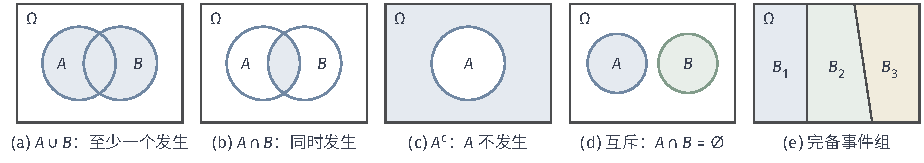
\includegraphics[width=156.5mm]{figures/01-basic-mathematics/05-probability-and-statistics-basics/tikz/prob-event-operations/figure.pdf}
  \caption{事件运算的集合示意。矩形表示样本空间$\Omega$，圆或分块表示事件，阴影是相应运算得到的事件。(a)(b)(c)分别是并、交与补；(d)中两个事件没有公共结果，因而互斥；(e)中三块互不重叠且铺满$\Omega$，每次试验恰有一块发生。}
  \label{fig:prob-event-operations}
\end{figure*}

\subsection{概率的定义与运算}
\label{sec:prob-probability-rules}

\paragraph{概率的定义}
我们希望给每个事件$A$配一个数$\mathbb{P}(A)$，表示它发生的可能性大小。直观上，这个数应当像“在大量重复试验中$A$发生的比例”那样运算：比例不会是负数，必然事件的比例是$1$，两个互斥事件合起来的比例等于各自比例之和。下面的定义只保留这三条规则，并把最后一条推广到可数个事件。

\begin{definition}[概率]
\label{def:prob-probability}
设对所讨论的每个事件$A$都给定一个实数$\mathbb{P}(A)$。若它满足
\begin{enumerate}
  \item 非负性：$\mathbb{P}(A)\geq0$；
  \item 归一性：$\mathbb{P}(\Omega)=1$；
  \item 可数可加性：对两两互斥的事件$A_1,A_2,\dots$，有$\mathbb{P}\bigl(\bigcup_{i\geq1}A_i\bigr)=\sum_{i\geq1}\mathbb{P}(A_i)$，
\end{enumerate}
就称$\mathbb{P}$为\term{概率}（probability），$\mathbb{P}(A)$为事件$A$的概率。
\end{definition}

第三条中的级数各项非负，它的和与求和次序无关（第~\ref{sec:ru-series-rearrangement-grouping}节）。为什么要求可数个而不只是有限个？等待时间问题中，“等待超过$10$分钟”可以拆成“等待落在$(10,11]$”“落在$(11,12]$”等可数个互斥事件之并；只有可数可加性，才能保证把这些片段的概率加起来得到整体的概率。

\paragraph{由定义推出的运算规则}
三条规则已经足以推出日常计算所需的公式。

\begin{theorem}[概率的基本性质]
\label{thm:prob-basic-properties}
设$A,B$为事件，则
\begin{enumerate}
  \item $\mathbb{P}(\varnothing)=0$，且对两两互斥的有限个事件有$\mathbb{P}(A_1\cup\dots\cup A_n)=\sum_{i=1}^n\mathbb{P}(A_i)$；
  \item 补事件公式：$\mathbb{P}(A^{\mathsf c})=1-\mathbb{P}(A)$；
  \item 单调性：若$A\subseteq B$，则$\mathbb{P}(B\setminus A)=\mathbb{P}(B)-\mathbb{P}(A)$，从而$\mathbb{P}(A)\leq\mathbb{P}(B)\leq1$；
  \item 加法公式：$\mathbb{P}(A\cup B)=\mathbb{P}(A)+\mathbb{P}(B)-\mathbb{P}(A\cap B)$，从而$\mathbb{P}(A\cup B)\leq\mathbb{P}(A)+\mathbb{P}(B)$。
\end{enumerate}
\end{theorem}
\begin{proof}
取$A_1=\Omega$、$A_i=\varnothing$（$i\geq2$），它们两两互斥，可数可加性给出$1=1+\sum_{i\geq2}\mathbb{P}(\varnothing)$；各项非负，只能$\mathbb{P}(\varnothing)=0$。把有限个互斥事件后面补上无穷多个空集，再用可数可加性，便得到有限可加性。

$A$与$A^{\mathsf c}$互斥且并为$\Omega$，有限可加性给出$\mathbb{P}(A)+\mathbb{P}(A^{\mathsf c})=1$。若$A\subseteq B$，则$B=A\cup(B\setminus A)$是互斥的并，于是$\mathbb{P}(B)=\mathbb{P}(A)+\mathbb{P}(B\setminus A)\geq\mathbb{P}(A)$；取$B=\Omega$即得$\mathbb{P}(A)\leq1$。

最后，$A\cup B$可以写成互斥的三块$A\setminus B$、$A\cap B$、$B\setminus A$之并，而$A$是前两块之并，$B$是后两块之并。分别对三者用有限可加性，便有$\mathbb{P}(A\cup B)=\mathbb{P}(A)+\mathbb{P}(B)-\mathbb{P}(A\cap B)$。
\end{proof}

加法公式减去$\mathbb{P}(A\cap B)$，是因为两块的公共部分被$\mathbb{P}(A)$与$\mathbb{P}(B)$各算了一次；它是第~\ref{chap:counting}章容斥原理的概率版本。丢掉这一项得到的不等式，对事件个数归纳后可推广到多个事件：$\mathbb{P}(A_1\cup\dots\cup A_n)\leq\sum_i\mathbb{P}(A_i)$，称为\term{联合界}（union bound）。它不要求事件互斥或有任何关系，因而常用来控制“至少有一处出错”的概率。补事件公式则提示一种常用的计算策略：“至少一个”往往不如它的反面“一个也没有”好算。

\paragraph{有限等可能模型}
若样本空间有限，并且根据试验的对称性认为每个样本点出现的可能性相同，就得到\term{古典概型}（classical probability model）：
\[
  \mathbb{P}(A)=\frac{|A|}{|\Omega|},
\]
其中$|A|$表示集合$A$的元素个数。概率计算由此化为计数。可以验证它满足概率的三条规则：比值非负，$|\Omega|/|\Omega|=1$，互斥事件的元素个数可以相加。

等可能性是我们对试验作出的模型假设，不是从样本空间推出的结论。公平骰子的六个面对称，所以取每面概率$1/6$；但如果把“两枚骰子的点数和”作为样本点，取值$2,3,\dots,12$并不等可能：和为$2$只有一种出法$(1,1)$，和为$7$却有六种。正确的做法是以有序对$(i,j)$为样本点，$36$个有序对等可能，于是点数和为$7$的概率是$6/36=1/6$，为$2$的概率只有$1/36$。

\begin{example}[抽检中至少一件次品]
\label{ex:prob-inspection-hypergeometric}
一批产品共$100$件，其中$5$件为次品。随机抽取$10$件且不放回，“随机”指$\binom{100}{10}$个$10$件子集等可能。样本中没有次品，等价于$10$件全部取自$95$件合格品，共有$\binom{95}{10}$种取法，所以
\[
  \mathbb{P}(\text{没有次品})=\frac{\binom{95}{10}}{\binom{100}{10}}
  =\frac{95\cdot94\cdots86}{100\cdot99\cdots91}\approx0.5838 .
\]
由补事件公式，至少抽到一件次品的概率约为$1-0.5838=0.4162$。也就是说，即使这批产品有$5\%$的次品，抽检$10$件仍有超过一半的可能一件次品也查不出来。
\end{example}

\paragraph{概率的连续性}
等待时间问题中，事件“$T<10$”可以由一列事件“$T\leq10-1/n$”逐步逼近，事件“$T\leq10$”也是“$T\leq10+1/n$”逐步收缩的极限。我们希望概率随事件的这种单调逼近而连续变化。若$A_1\subseteq A_2\subseteq\cdots$且$A=\bigcup_nA_n$，记作$A_n\uparrow A$；若$A_1\supseteq A_2\supseteq\cdots$且$A=\bigcap_nA_n$，记作$A_n\downarrow A$。

\begin{theorem}[概率的连续性]
\label{thm:prob-continuity}
若$A_n\uparrow A$，则$\mathbb{P}(A_n)\to\mathbb{P}(A)$；若$A_n\downarrow A$，同样有$\mathbb{P}(A_n)\to\mathbb{P}(A)$。
\end{theorem}
\begin{proof}
设$A_n\uparrow A$。令$B_1=A_1$，$B_n=A_n\setminus A_{n-1}$（$n\geq2$），即$B_n$是第$n$步新增加的部分。这些$B_n$两两互斥，$A_n=B_1\cup\dots\cup B_n$，且$A=\bigcup_{n\geq1}B_n$。由可数可加性与有限可加性，
\[
  \mathbb{P}(A)=\sum_{k=1}^{\infty}\mathbb{P}(B_k)
  =\lim_{n\to\infty}\sum_{k=1}^{n}\mathbb{P}(B_k)
  =\lim_{n\to\infty}\mathbb{P}(A_n).
\]
若$A_n\downarrow A$，则补事件满足$A_n^{\mathsf c}\uparrow A^{\mathsf c}$（De Morgan律），由前一结论$\mathbb{P}(A_n^{\mathsf c})\to\mathbb{P}(A^{\mathsf c})$，再用补事件公式即得。
\end{proof}

证明中递减情形借助了补事件，这里用到$\mathbb{P}(\Omega)=1$有限。连续性是可数可加性的直接推论；下一节将用它说明分布函数为什么右连续，以及单点概率怎样由分布函数的跳跃读出。

\subsection{条件概率}
\label{sec:prob-conditional-probability}

\paragraph{定义与直观}
掷一枚公平骰子，“点数不小于$4$”的概率是$1/2$。若有人告诉我们这次出现的是偶数点，可能的结果就只剩$\{2,4,6\}$，其中$4$和$6$两个满足条件，可能性变成$2/3$。已知信息把考虑范围从$\Omega$缩小到事件$B$，再在$B$内部按原来的相对大小重新分配概率。

\begin{definition}[条件概率]
\label{def:prob-conditional-probability}
设$\mathbb{P}(B)>0$。事件$A$在事件$B$发生条件下的\term{条件概率}（conditional probability）定义为
\[
  \mathbb{P}(A\mid B)=\frac{\mathbb{P}(A\cap B)}{\mathbb{P}(B)} .
\]
\end{definition}

分子只保留$A$中同时落在$B$内的部分，分母$\mathbb{P}(B)$把$B$的总概率重新标定为$1$。在古典概型中，它就是$|A\cap B|/|B|$，即只在$B$内部计数。固定$B$后，$A\mapsto\mathbb{P}(A\mid B)$本身满足概率的三条规则，因此前面的补事件公式、加法公式等都可以在条件之下照用。定义要求$\mathbb{P}(B)>0$：以零概率事件为条件需要另外的构造，本节不讨论；对连续取值变量取条件的问题，留到第~\ref{sec:rvec-conditioning}节用条件密度处理。

\paragraph{乘法公式}
把定义式两边乘以$\mathbb{P}(B)$，得到\term{乘法公式}（multiplication rule）
\[
  \mathbb{P}(A\cap B)=\mathbb{P}(B)\,\mathbb{P}(A\mid B).
\]
它适合按时间顺序计算：先算第一步的概率，再乘以在第一步结果已知时第二步的条件概率。对多个事件反复使用，只要各个条件事件的概率为正，就有
\[
  \mathbb{P}(A_1\cap A_2\cap\dots\cap A_n)
  =\mathbb{P}(A_1)\,\mathbb{P}(A_2\mid A_1)\cdots\mathbb{P}(A_n\mid A_1\cap\dots\cap A_{n-1}).
\]

\begin{example}[不放回抽球]
\label{ex:prob-urn-without-replacement}
袋中有$3$个红球、$2$个白球，依次不放回地摸出两个。记$R_1$、$R_2$分别为第一、二次摸到红球。第一次摸到红球后袋中剩$2$红$2$白，所以$\mathbb{P}(R_2\mid R_1)=2/4$；第一次摸到白球后剩$3$红$1$白，所以$\mathbb{P}(R_2\mid R_1^{\mathsf c})=3/4$。由乘法公式，
\[
  \mathbb{P}(R_1\cap R_2)=\frac35\cdot\frac24=\frac{3}{10},\qquad
  \mathbb{P}(R_1^{\mathsf c}\cap R_2)=\frac25\cdot\frac34=\frac{3}{10}.
\]
两者互斥且并为$R_2$，故$\mathbb{P}(R_2)=3/5$，与第一次摸到红球的概率相同。

不放回时，第一次的结果改变了第二次的条件概率：$1/2$与$3/4$都不等于$3/5$。若每次摸完放回，袋中构成不变，无论第一次摸到什么，第二次摸到红球的条件概率都是$3/5$。条件是否改变后续概率，正是下一小节要刻画的独立性。
\end{example}

\subsection{事件的独立性}
\label{sec:prob-event-independence}

\paragraph{两个事件的独立}
放回抽球时，第一次的结果不改变第二次的概率：$\mathbb{P}(R_2\mid R_1)=\mathbb{P}(R_2)$。把这一等式乘以$\mathbb{P}(R_1)$，就得到对称的乘积形式，它在$\mathbb{P}(R_1)=0$时也有意义。

\begin{definition}[事件的独立性]
\label{def:prob-independent-events}
若$\mathbb{P}(A\cap B)=\mathbb{P}(A)\,\mathbb{P}(B)$，就称事件$A$与$B$\term{相互独立}（independent）。
\end{definition}

当$\mathbb{P}(B)>0$时，独立等价于$\mathbb{P}(A\mid B)=\mathbb{P}(A)$，即知道$B$发生并不改变$A$的概率。若$A$与$B$独立，则$A$与$B^{\mathsf c}$也独立：$\mathbb{P}(A\cap B^{\mathsf c})=\mathbb{P}(A)-\mathbb{P}(A\cap B)=\mathbb{P}(A)(1-\mathbb{P}(B))=\mathbb{P}(A)\mathbb{P}(B^{\mathsf c})$。“$B$发生”不提供关于$A$的信息，“$B$不发生”同样不提供。

独立性是关于概率数值的条件，要按定义核对，不能凭事件“看起来无关”判断。掷一枚公平骰子，令$A=\{2,4,6\}$，$B=\{1,2\}$，$C=\{1,2,3\}$。$\mathbb{P}(A\cap B)=\mathbb{P}(\{2\})=1/6=\frac12\cdot\frac13$，所以$A$与$B$独立；$\mathbb{P}(A\cap C)=1/6\neq\frac12\cdot\frac12$，所以$A$与$C$不独立。独立也不同于互斥：若$\mathbb{P}(A),\mathbb{P}(B)>0$且$A,B$互斥，则$\mathbb{P}(A\cap B)=0<\mathbb{P}(A)\mathbb{P}(B)$，知道$B$发生就确知$A$不发生，二者并不独立。

\paragraph{多个事件的相互独立}
三个以上事件的独立性要更小心。我们希望任意几个事件的发生情况都不影响其余事件，这需要所有子组都满足乘法关系。

\begin{definition}[多个事件的相互独立]
\label{def:prob-mutual-independence}
称事件$A_1,\dots,A_n$相互独立（mutually independent），若对任意$2\leq k\leq n$和任意下标$1\leq i_1<\dots<i_k\leq n$，都有
\[
  \mathbb{P}(A_{i_1}\cap\dots\cap A_{i_k})=\mathbb{P}(A_{i_1})\cdots\mathbb{P}(A_{i_k}).
\]
\end{definition}

只验证两两之间的乘法关系是不够的。

\begin{example}[两两独立但不相互独立]
\label{ex:prob-pairwise-not-mutual}
抛两枚公平硬币，四个结果等可能。令$A$为“第一枚正面”，$B$为“第二枚正面”，$C$为“两枚结果相同”。每个事件的概率都是$1/2$，任意两个同时发生的概率都是$1/4$（例如$A\cap C$就是“两枚都正面”），所以三对事件都独立。但$A\cap B$发生时$C$必然发生，$\mathbb{P}(A\cap B\cap C)=1/4\neq1/8$，三者不相互独立：知道$A$与$B$，就完全知道了$C$。
\end{example}

相互独立的定义为“独立重复试验”给出了明确条件。设一项试验重复$n$次，$A_i$是只依赖第$i$次结果的事件（例如“第$i$次成功”）。若$A_1,\dots,A_n$相互独立，且$\mathbb{P}(A_i)=p$，则$n$次全部成功的概率是$p^n$，前$k$次成功、其余失败的概率是$p^k(1-p)^{n-k}$（独立性对补事件保持，可以把其中任意几个$A_i$换成补事件）。第~\ref{sec:prob-discrete-models}节的二项分布与几何分布都建立在这个条件上。

\section{随机变量与概率分布}
\label{sec:prob-distributions}

抽检关心次品的“个数”，排队关心等待的“分钟数”。我们常常不需要试验结果的全部细节，只需要由结果算出的一个数。本节把这种“结果到数值”的对应写成随机变量，并研究怎样完整描述它取各种值的概率。

\subsection{随机变量与实现值}
\label{sec:prob-random-variables}

\paragraph{随机变量}
抽检的样本点是一个$10$件子集，而我们关心的是其中次品的个数；这个个数由样本点完全确定，但样本点本身是随机的。把每个结果对应到一个实数的规则，就是随机变量。

\begin{definition}[随机变量]
\label{def:prob-random-variable}
定义在样本空间上的实值函数$X:\Omega\to\mathbb{R}$称为\term{随机变量}（random variable）。对实数集的子集$B$，记
\[
  \{X\in B\}=\{\omega\in\Omega: X(\omega)\in B\},
\]
它是一个事件，其概率记作$\mathbb{P}(X\in B)$。
\end{definition}

本部分默认所讨论的$\{X\in B\}$（$B$为区间或单点等）都是可以赋予概率的事件；一般的可测性要求见\BookPartRef{part:probability-spaces}{卷2《数学准备：抽象数学》的“概率空间”部分}。随机变量本身是一个确定的函数，随机性来自样本点$\omega$的出现。我们把随机变量记成大写字母$X$，它的可能取值组成集合$X(\Omega)$；一次试验出现结果$\omega$后，得到的具体数$x=X(\omega)$称为$X$的一个\term{实现值}（realization），用小写字母表示。例如“$X\leq3$”是一个事件，而“$x=2$”是一次观测的结果。

\paragraph{分布由映射与概率共同决定}
同一次试验可以定义多个随机变量。掷一枚骰子，$\Omega=\{1,\dots,6\}$，令$X(\omega)=\omega$为点数，令
\[
  I(\omega)=\begin{cases}1,&\omega\text{为偶数},\\0,&\omega\text{为奇数}.\end{cases}
\]
$I$只记录点数的奇偶。一般地，对事件$A$，称取值$1$（$\omega\in A$）或$0$（$\omega\notin A$）的函数$\mathbb{I}_A$为$A$的\term{指示函数}（indicator function），于是$I=\mathbb{I}_{\{2,4,6\}}$。图~\ref{fig:prob-die-indicator-map}画出了两个变量的对应关系：$X$把六个结果送到六个不同的值，$I$则把三个偶数结果合并到$1$，三个奇数结果合并到$0$。

\begin{figure}[htbp]
  \centering
  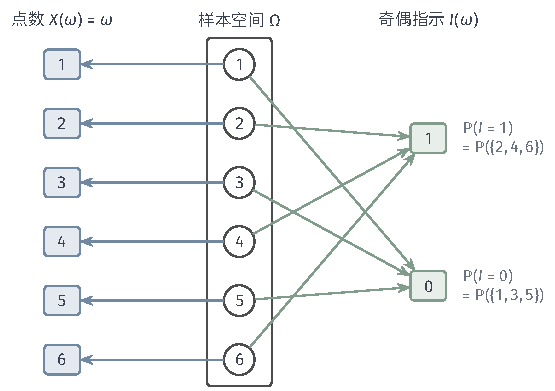
\includegraphics[width=94mm]{figures/01-basic-mathematics/05-probability-and-statistics-basics/tikz/prob-die-indicator-map/figure.pdf}
  \caption{同一次掷骰试验上的两个随机变量。中间是样本空间的六个结果；左侧的点数$X$把每个结果送到不同的值，右侧的奇偶指示变量$I$把三个偶数结果都送到$1$、三个奇数结果都送到$0$。$I$取某个值的概率，等于被送到该值的全部结果的概率之和。}
  \label{fig:prob-die-indicator-map}
\end{figure}

要知道$I$取$1$的概率，就把被送到$1$的结果的概率加起来：$\mathbb{P}(I=1)=\mathbb{P}(\{2,4,6\})$。骰子公平时它等于$1/2$。若骰子被做了手脚，$\mathbb{P}(\{6\})=1/2$，其余五面各为$1/10$，同一个函数$I$给出$\mathbb{P}(I=1)=0.1+0.1+0.5=0.7$。可见随机变量取值的概率规律既取决于对应规则$X$，也取决于试验结果上的概率$\mathbb{P}$。

\begin{definition}[分布]
\label{def:prob-distribution}
随机变量$X$的\term{分布}（distribution）是指对实数集的各个子集$B$给出概率$\mathbb{P}(X\in B)$的对应关系$B\mapsto\mathbb{P}(X\in B)$，也记作$P_X(B)$。
\end{definition}

分布只记录“取值落在哪里的概率”，不再记录是哪个结果导致了这个取值。不同的随机变量可以有相同的分布：公平骰子上的$I$与$1-I$（奇数指示）都以概率$1/2$取$0$和$1$，但在每次试验中二者的取值恰好相反。所以“分布相同”与“随机变量相等”是两回事；两个随机变量$X,Y$分布相同时，记作$X\overset{d}{=}Y$，以区别于逐个结果都相等的$X=Y$。

\subsection{分布函数}
\label{sec:prob-cdf}

\paragraph{定义与性质}
分布要对很多集合给出概率，逐一列出并不现实。对实值随机变量，只需记录形如$(-\infty,x]$的半直线的概率，其余区间的概率就能由它们相减得到。

\begin{definition}[分布函数]
\label{def:prob-cdf}
随机变量$X$的\term{分布函数}（distribution function，也称累积分布函数，cumulative distribution function，CDF）定义为
\[
  F_X(x)=\mathbb{P}(X\leq x),\qquad x\in\mathbb{R}.
\]
\end{definition}

对$a<b$，事件$\{X\leq b\}$是互斥的$\{X\leq a\}$与$\{a<X\leq b\}$之并，因此
\[
  \mathbb{P}(a<X\leq b)=F_X(b)-F_X(a).
\]
左开右闭的区间与分布函数的“$\leq$”配套。其他类型区间的概率还需要知道单点概率，这由下面的性质给出。

\begin{theorem}[分布函数的性质]
\label{thm:prob-cdf-properties}
任一随机变量的分布函数$F=F_X$满足：
\begin{enumerate}
  \item 单调不减：$x<y$时$F(x)\leq F(y)$；
  \item 右连续：$\lim_{y\downarrow x}F(y)=F(x)$；
  \item 两端极限：$\lim_{x\to-\infty}F(x)=0$，$\lim_{x\to+\infty}F(x)=1$。
\end{enumerate}
此外，左极限$F(x^-)=\lim_{y\uparrow x}F(y)$存在，且$F(x^-)=\mathbb{P}(X<x)$，$\mathbb{P}(X=x)=F(x)-F(x^-)$。
\end{theorem}
\begin{proof}
$x<y$时$\{X\leq x\}\subseteq\{X\leq y\}$，单调性由概率的单调性得到。单调函数的单侧极限总存在，所以只需沿特殊数列计算极限。

取$y_n=x+1/n$，事件$\{X\leq y_n\}$递减，交集为$\{X\leq x\}$，由概率的连续性$F(y_n)\to F(x)$，这就是右连续。同理，$\{X\leq -n\}\downarrow\varnothing$，$\{X\leq n\}\uparrow\Omega$，分别给出两端极限$0$与$1$。

最后取$y_n=x-1/n$，事件$\{X\leq y_n\}$递增，并集是$\{X<x\}$（不含$x$本身），所以$F(x^-)=\mathbb{P}(X<x)$。$\{X\leq x\}$是$\{X<x\}$与$\{X=x\}$的互斥并，相减即得单点概率。
\end{proof}

右连续而不一定左连续的原因在于“$\leq$”包含端点：从右侧逼近$x$的事件交出$\{X\leq x\}$，从左侧逼近的事件并出$\{X<x\}$，二者相差的正是单点$\{X=x\}$。于是分布函数在$x$处的跳跃高度等于$\mathbb{P}(X=x)$，而$F$在$x$连续当且仅当$\mathbb{P}(X=x)=0$。有了单点概率，$\mathbb{P}(a\leq X\leq b)=F(b)-F(a^-)$等各类区间的概率都能写出。反过来也成立：任何满足上述三条性质的函数，都是某个随机变量的分布函数，并且分布函数唯一确定分布；这一结论的证明需要一般测度构造，留到\BookPartRef{part:probability-spaces}{卷2《数学准备：抽象数学》的“概率空间”部分}。

\paragraph{三类分布函数}
分布函数对所有实值随机变量都有定义，因而能用同一种语言描述取值方式很不相同的变量。下面三个例子对应图~\ref{fig:prob-cdf-three-types}的三幅子图。

\begin{figure*}[htbp]
  \centering
  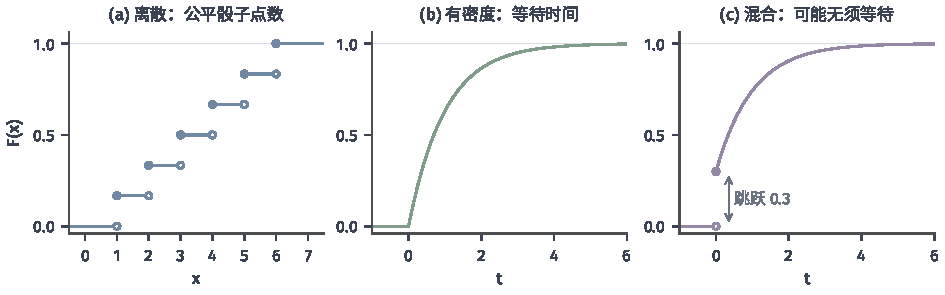
\includegraphics[width=160mm]{figures/01-basic-mathematics/05-probability-and-statistics-basics/matplotlib/prob-cdf-three-types/figure.pdf}
  \caption{三类分布函数。(a)公平骰子的点数，分布函数是阶梯函数，在$1,\dots,6$各跳$1/6$，实心点表示取到的函数值、空心点表示左极限；(b)等待时间$T$满足$F(t)=1-e^{-t}$（$t\geq0$），曲线连续；(c)以概率$0.3$无须等待、否则等待时间按(b)的规律分布，曲线在$0$处跳跃$0.3$，之后连续上升。三条曲线都单调不减、右连续，并从$0$升到$1$。}
  \label{fig:prob-cdf-three-types}
\end{figure*}

\begin{example}[离散、连续与混合]
\label{ex:prob-three-cdfs}
(a)公平骰子的点数$X$：$x<1$时$F_X(x)=0$，$k\leq x<k+1$（$k=1,\dots,5$）时$F_X(x)=k/6$，$x\geq6$时$F_X(x)=1$。函数在每个整数点$k$跳跃$1/6$，在两个整数之间保持水平。

(b)等待时间$T$满足$F_T(t)=0$（$t<0$）、$F_T(t)=1-e^{-t}$（$t\geq0$），以分钟计。它处处连续，所以每个单点的概率都是$0$；等待超过$2$分钟的概率是$1-F_T(2)=e^{-2}\approx0.135$。

(c)设窗口空闲时（概率$0.3$）顾客无须等待，否则等待时间按(b)的规律分布。于是
\[
  F_W(t)=\begin{cases}0,&t<0,\\0.3+0.7(1-e^{-t}),&t\geq0.\end{cases}
\]
函数在$0$处跳跃$0.3$，即$\mathbb{P}(W=0)=0.3$；在$t>0$上连续上升。
\end{example}

例(a)的变量只取有限个值，概率全部集中在这些点上；例(b)的变量没有任何单点带正概率；例(c)两者兼有。接下来的两小节分别为前两类给出更方便的表示：概率质量函数和概率密度函数。例(c)说明这两类并不覆盖全部情形，此时分布函数仍然适用，计算可以把跳跃部分求和、连续部分积分。

\subsection{概率质量函数}
\label{sec:prob-pmf}

\paragraph{定义与计算}
骰子点数、次品个数这类变量只取有限或可数多个值。对它们而言，最直接的描述是逐个列出每个取值的概率。

\begin{definition}[离散随机变量与概率质量函数]
\label{def:prob-pmf}
若存在有限或可数的集合$\{x_1,x_2,\dots\}$使$\mathbb{P}(X\in\{x_1,x_2,\dots\})=1$，就称$X$为\term{离散随机变量}（discrete random variable）。函数
\[
  p_X(x)=\mathbb{P}(X=x),\qquad x\in\mathbb{R}
\]
称为$X$的\term{概率质量函数}（probability mass function，PMF）。
\end{definition}

质量函数满足$p_X(x)\geq0$，只在可能取值处为正，且$\sum_ip_X(x_i)=1$。对任意集合$B$，事件$\{X\in B\}$是可数个互斥单点事件$\{X=x_i\}$（$x_i\in B$）之并，由可数可加性
\[
  \mathbb{P}(X\in B)=\sum_{x_i\in B}p_X(x_i).
\]
反过来，任给可数个点和满足非负、总和为$1$的一组数，都能定义一个离散分布。离散分布的计算因而就是求和。

\begin{example}[三次抛硬币的正面数]
\label{ex:prob-three-coins}
抛三枚公平硬币，令$X$为正面个数。$8$个结果等可能，含$k$个正面的结果有$\binom{3}{k}$个，所以
\[
  p_X(0)=\tfrac18,\quad p_X(1)=\tfrac38,\quad p_X(2)=\tfrac38,\quad p_X(3)=\tfrac18 .
\]
“至少一次正面”的概率是$p_X(1)+p_X(2)+p_X(3)=7/8$，也可以用补事件写成$1-p_X(0)$。
\end{example}

\paragraph{质量函数与分布函数}
离散变量的分布函数是质量函数的累加：
\[
  F_X(x)=\sum_{x_i\leq x}p_X(x_i).
\]
因此$F_X$是阶梯函数，跳跃发生在可能取值$x_i$处，跳跃高度就是$p_X(x_i)$，这正是定理~\ref{thm:prob-cdf-properties}中$\mathbb{P}(X=x)=F(x)-F(x^-)$的具体形式。图~\ref{fig:prob-pmf-cdf}把例~\ref{ex:prob-three-coins}的两种表示并排画出：左图的竖线高度，正是右图对应台阶的高度差。

\begin{figure}[htbp]
  \centering
  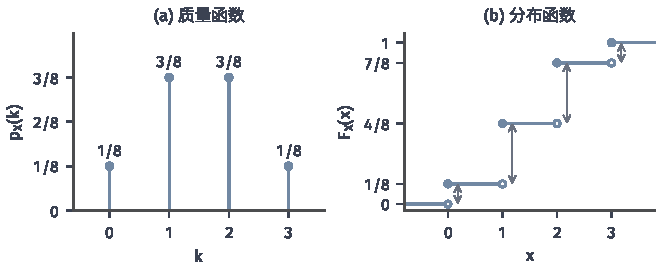
\includegraphics[width=112mm]{figures/01-basic-mathematics/05-probability-and-statistics-basics/matplotlib/prob-pmf-cdf/figure.pdf}
  \caption{三次抛公平硬币的正面数。(a)概率质量函数，竖线高度是各取值的概率；(b)分布函数，箭头标出每个台阶的跳跃高度，依次为$1/8,3/8,3/8,1/8$，与(a)的竖线一一对应。两次跳跃之间分布函数保持水平，因为那里没有可能取值。}
  \label{fig:prob-pmf-cdf}
\end{figure}

两种表示可以互相转换：从质量函数累加得到分布函数，从分布函数读出各处的跳跃得到质量函数。计算区间概率时，分布函数往往更快：$\mathbb{P}(1\leq X\leq2)=F_X(2)-F_X(1^-)=F_X(2)-F_X(0)=7/8-1/8=3/4$。注意这里用的是$F_X(1^-)$而不是$F_X(1)$，因为区间包含左端点$1$，而$1$处恰有正概率。

\subsection{概率密度函数}
\label{sec:prob-pdf}

\paragraph{用积分计算概率}
等待时间的每个单点概率都是$0$，质量函数不能提供任何信息。此时我们改用“单位长度上的概率”来描述：概率像质量一样沿数轴连续分布，区间上的概率是密度在该区间上的积分。

\begin{definition}[概率密度函数]
\label{def:prob-pdf}
若存在非负函数$f_X$，使$\int_{-\infty}^{\infty}f_X(x)\,\mathrm{d}x=1$，并且对一切$a<b$都有
\[
  \mathbb{P}(a<X\leq b)=\int_a^b f_X(x)\,\mathrm{d}x,
\]
就称$X$具有\term{概率密度函数}（probability density function，PDF）$f_X$，简称密度。
\end{definition}

这里的积分可以是第~\ref{sec:ru-improper-integrals}节的反常积分，$a$也可以取$-\infty$。有密度的变量满足$\mathbb{P}(X=x)=0$：分布函数$F_X(x)=\int_{-\infty}^xf_X(t)\,\mathrm{d}t$是积分上限函数，处处连续，而由定理~\ref{thm:prob-cdf-properties}，单点概率就是分布函数在该点的跳跃高度。因此$\mathbb{P}(a<X\leq b)$、$\mathbb{P}(a\leq X\leq b)$、$\mathbb{P}(a<X<b)$都相等，端点开闭不影响结果。

密度值不是概率。若$f_X$在$x$处连续，由积分中值定理，
\[
  \mathbb{P}(x<X\leq x+h)=\int_x^{x+h}f_X(t)\,\mathrm{d}t\approx f_X(x)\,h,
\]
更准确地说，中值定理给出$\int_x^{x+h}f_X=f_X(\xi_h)h$，其中$\xi_h\in[x,x+h]$，由连续性$f_X(\xi_h)\to f_X(x)$。所以$f_X(x)$是“小区间上的概率除以区间长度”的极限，单位是“概率每单位长度”。它可以大于$1$，只要乘上区间长度后的累计不超过$1$。

\begin{example}[密度值大于一]
\label{ex:prob-density-above-one}
设$X$在$(0,1/2)$上取值，且等长子区间等可能，则$f_X(x)=2$（$0<x<1/2$），其余处为$0$。密度处处等于$2$，但$\mathbb{P}(0.1<X\leq0.3)=2\times0.2=0.4$。又设等待时间$T$的密度为$f_T(t)=3e^{-3t}$（$t\geq0$），则$f_T(0)=3$，而$\mathbb{P}(0<T\leq0.2)=1-e^{-0.6}\approx0.451$。图~\ref{fig:prob-density-above-one}画出这两个密度，阴影面积就是所求概率。
\end{example}

\begin{figure}[htbp]
  \centering
  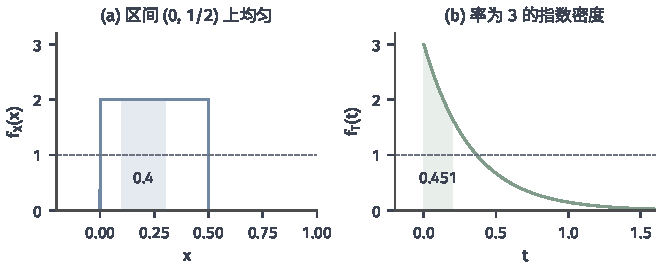
\includegraphics[width=112mm]{figures/01-basic-mathematics/05-probability-and-statistics-basics/matplotlib/prob-density-above-one/figure.pdf}
  \caption{密度值可以大于一。(a)区间$(0,1/2)$上的均匀密度恒为$2$，阴影是$\mathbb{P}(0.1<X\leq0.3)=0.4$；(b)率为$3$的指数密度在$0$处等于$3$，阴影是$\mathbb{P}(0<T\leq0.2)\approx0.451$。虚线标出高度$1$。概率由面积给出，曲线的高度只表示单位长度上的概率。}
  \label{fig:prob-density-above-one}
\end{figure}

\paragraph{密度与分布函数}
取$a\to-\infty$，定义直接给出分布函数是密度的累计：
\[
  F_X(x)=\int_{-\infty}^{x}f_X(t)\,\mathrm{d}t .
\]
由微积分基本定理（定理~\ref{thm:ru-accumulation-derivative}），在$f_X$连续的点有$F_X'(x)=f_X(x)$：密度是分布函数的变化率。反过来，若$F_X$连续，并且除有限个点外连续可微，那么$f_X=F_X'$（在那有限个点处任意取值）就是一个密度，因为由Newton--Leibniz公式，每段上$F_X$的增量都等于$F_X'$的积分，而有限个点不影响积分。例如$F_X(x)=x^2$（$0\leq x\leq1$）连同两侧的$0$与$1$，给出密度$f_X(x)=2x$（$0<x<1$）。

密度只在积分意义下确定：改变有限个点处的函数值，所有区间上的积分都不变，所以两个密度若只在有限个点不同，描述的是同一个分布。另一方面，“分布函数连续”还不足以保证密度存在。有连续分布函数的变量所有单点概率为零，但仍可能把全部概率集中在一个“总长度为零”的集合上；Cantor函数就是这样的例子，它连续、单调地从$0$升到$1$，导数却在除一个零长度集合外的所有点都等于零，任何密度的积分都无法还原它。这类分布在应用中很少直接出现，但它说明离散分布与有密度的分布并未穷尽所有情形，例~\ref{ex:prob-three-cdfs}(c)的混合分布也不属于这两类。

\section{分布的数值特征}
\label{sec:prob-numerical-features}

分布函数、质量函数和密度保存了分布的全部信息，但回答“平均要等多久”“波动有多大”这类问题时，我们需要的是一两个数。本节用期望描述平均位置，用方差描述围绕平均的波动，用分位数描述累计概率对应的位置，再用高阶矩补充形状信息。

\subsection{期望}
\label{sec:prob-expectation}

\paragraph{定义与可积条件}
掷一枚公平骰子很多次，点数的平均值会稳定在什么地方？每个点数出现的比例约为$1/6$，平均值就约为$\sum_{k=1}^6k\cdot\frac16=3.5$。这个计算把每个可能取值按其概率加权平均，它不依赖任何一次的具体结果。重复次数增加时样本平均为何会接近这个数，是第~\ref{sec:samp-lln}节大数定律的内容；这里先把加权平均本身定义清楚。

\begin{definition}[期望]
\label{def:prob-expectation}
设$X$为离散随机变量，质量函数为$p_X$。若级数$\sum_i|x_i|\,p_X(x_i)$收敛，定义$X$的\term{期望}（expectation）为
\[
  \mathbb{E}[X]=\sum_ix_i\,p_X(x_i).
\]
设$X$具有密度$f_X$。若$\int_{-\infty}^{\infty}|x|\,f_X(x)\,\mathrm{d}x<\infty$，定义
\[
  \mathbb{E}[X]=\int_{-\infty}^{\infty}x\,f_X(x)\,\mathrm{d}x .
\]
满足相应条件时，称$X$的期望有限，或称$X$\term{可积}（integrable）。期望也称\term{均值}（mean），常记作$\mu$或$\mu_X$。
\end{definition}

定义先要求绝对值的加权和有限，是因为可数个取值可能有正有负。若只是条件收敛，第~\ref{sec:ru-series-rearrangement-grouping}节已经说明重排求和次序可以改变级数的和，而可能取值并没有天然的先后次序；绝对收敛保证无论按什么次序相加结果都一样。对非负变量，加权和要么有限、要么为$+\infty$，此时可以写$\mathbb{E}[X]=+\infty$；对一般变量，绝对值的和无穷时期望没有定义。

\begin{example}[期望不存在的分布]
\label{ex:prob-infinite-expectation}
设$X$取正整数，$p_X(k)=\frac{1}{k(k+1)}$。由$\frac{1}{k(k+1)}=\frac1k-\frac1{k+1}$，部分和逐项相消，$\sum_{k\geq1}p_X(k)=1$，这是一个合法的分布。但$\sum_kk\,p_X(k)=\sum_k\frac{1}{k+1}=+\infty$，所以$\mathbb{E}[X]=+\infty$：大的取值概率虽小，衰减却不够快。连续情形的例子是Cauchy密度$f(x)=\frac{1}{\pi(1+x^2)}$，它关于$0$对称，但$\int|x|f(x)\,\mathrm{d}x=+\infty$，期望没有定义，不能凭对称性说期望等于$0$。
\end{example}

例~\ref{ex:prob-three-cdfs}(c)的混合分布兼有跳跃与连续部分，其期望把两部分分别计算后相加：$\mathbb{E}[W]=0\times0.3+\int_0^\infty t\cdot0.7e^{-t}\,\mathrm{d}t=0.7$。一般分布统一的期望定义需要测度积分，留到\BookPartRef{part:probability-spaces}{卷2《数学准备：抽象数学》的“概率空间”部分}；本部分只用离散求和与密度积分。

\paragraph{函数的期望与线性性}
我们常常需要$X$的某个函数的平均，例如点数平方的平均，或观测加上噪声后的平均。按定义，似乎要先求出新变量$g(X)$的分布，再求加权平均。下面的结论说明这一步可以省去。

\begin{theorem}[函数的期望]
\label{thm:prob-lotus}
设$g$为实值函数。若$X$离散，且级数$\sum_i|g(x_i)|\,p_X(x_i)$收敛，则
\[
  \mathbb{E}[g(X)]=\sum_ig(x_i)\,p_X(x_i);
\]
若$X$有密度$f_X$，$g$分段连续且$\int|g(x)|f_X(x)\,\mathrm{d}x<\infty$，则
\begin{equation}
  \mathbb{E}[g(X)]=\int_{-\infty}^{\infty}g(x)\,f_X(x)\,\mathrm{d}x .
  \label{eq:prob-lotus}
\end{equation}
\end{theorem}
\begin{proof}
只证离散情形。$Y=g(X)$也是离散变量，它取值$y$当且仅当$X$取某个满足$g(x_i)=y$的$x_i$，所以$p_Y(y)=\sum_{i:\,g(x_i)=y}p_X(x_i)$。按$Y$的定义，
\[
  \mathbb{E}[Y]=\sum_yy\,p_Y(y)=\sum_y\sum_{i:\,g(x_i)=y}g(x_i)\,p_X(x_i)=\sum_ig(x_i)\,p_X(x_i).
\]
最后一步把双重和按$i$重新排列：每个$i$恰好出现在$y=g(x_i)$那一组中。绝对收敛的假设保证重排不改变和，同时也说明$Y$的期望有限。
\end{proof}

密度情形的证明需要知道$g(X)$的分布。第~\ref{sec:prob-density-change}节在$g$严格单调可微时用变量替换验证式~\eqref{eq:prob-lotus}；一般情形的证明留到\BookPartRef{part:probability-spaces}{卷2《数学准备：抽象数学》的“概率空间”部分}。例如公平骰子点数的平方，直接计算$\mathbb{E}[X^2]=\frac16(1+4+9+16+25+36)=\frac{91}{6}$，不必先列出$X^2$取$1,4,\dots,36$的分布。

由定理~\ref{thm:prob-lotus}与求和、积分的线性性，期望对函数的线性组合是线性的：只要$g(X)$与$h(X)$的期望都有限，对常数$a,b,c$有
\[
  \mathbb{E}[a\,g(X)+b\,h(X)+c]=a\,\mathbb{E}[g(X)]+b\,\mathbb{E}[h(X)]+c .
\]
特别地，$\mathbb{E}[aX+b]=a\,\mathbb{E}[X]+b$，常数的期望是它自己。多个不同随机变量之和的期望同样可以拆开，其证明要用到它们的联合分布，在第~\ref{sec:rvec-moments}节讨论。

\begin{example}[带噪观测的平均目标]
\label{ex:probability-noisy-observation}
用仪器测量一个固定的未知量$\theta$，读数为$Y=\theta+\varepsilon$，其中误差$\varepsilon$是随机变量，满足$\mathbb{E}[\varepsilon]=0$。$Y$是$\varepsilon$的函数$g(\varepsilon)=\theta+\varepsilon$，由线性性
\[
  \mathbb{E}[Y]=\theta+\mathbb{E}[\varepsilon]=\theta .
\]
这说明读数“平均而言”没有系统偏差，却不保证一次读数接近$\theta$。例如$\varepsilon$以各$1/2$的概率取$\pm10$，则$\mathbb{E}[Y]=\theta$，但每次读数都恰好偏离$\theta$十个单位。期望只描述平均位置；读数离$\theta$有多远，需要下一小节的方差来刻画，多次读数的平均能否接近$\theta$，则要等到第~\ref{chap:sampling-errors}章讨论。
\end{example}

\subsection{方差与标准差}
\label{sec:prob-variance}

\paragraph{定义与计算公式}
例~\ref{ex:probability-noisy-observation}中，误差取$\pm10$与取$\pm1$的期望都是$0$，读数的可靠程度却差别很大。要区分它们，需要衡量取值偏离均值的典型程度。偏差$X-\mu$有正有负，平均起来恰为零，所以我们取偏差的平方再平均。

\begin{definition}[方差与标准差]
\label{def:prob-variance}
设$\mathbb{E}[X^2]<\infty$，记$\mu=\mathbb{E}[X]$。$X$的\term{方差}（variance）定义为
\[
  \operatorname{Var}(X)=\mathbb{E}\bigl[(X-\mu)^2\bigr],
\]
其非负平方根$\sigma_X=\sqrt{\operatorname{Var}(X)}$称为\term{标准差}（standard deviation）。方差也常记作$\sigma^2$或$\sigma_X^2$。
\end{definition}

条件$\mathbb{E}[X^2]<\infty$称为二阶矩有限，它保证均值也有限：由$|x|\leq\frac12(1+x^2)$，$\mathbb{E}|X|\leq\frac12(1+\mathbb{E}[X^2])<\infty$。展开平方并用线性性，得到常用的计算公式
\[
  \operatorname{Var}(X)=\mathbb{E}[X^2]-2\mu\,\mathbb{E}[X]+\mu^2=\mathbb{E}[X^2]-\mu^2 .
\]
方差总是非负的，所以$\mathbb{E}[X^2]\geq(\mathbb{E}[X])^2$。方差为零意味着$X$以概率$1$等于常数$\mu$：对离散变量，$\sum_i(x_i-\mu)^2p_X(x_i)=0$要求每个正概率取值都等于$\mu$。

\begin{example}[骰子点数的方差]
\label{ex:prob-die-variance}
公平骰子的点数有$\mu=7/2$，$\mathbb{E}[X^2]=91/6$，于是
\[
  \operatorname{Var}(X)=\frac{91}{6}-\frac{49}{4}=\frac{182-147}{12}=\frac{35}{12}\approx2.92,
  \qquad \sigma_X\approx1.71 .
\]
对比例~\ref{ex:probability-noisy-observation}：误差取$\pm10$时$\operatorname{Var}(\varepsilon)=100$，取$\pm1$时为$1$，两者的标准差分别是$10$与$1$，正是典型偏离的大小。
\end{example}

\paragraph{单位与线性变换}
方差的单位是原变量单位的平方：等待时间以分钟计，方差的单位就是“平方分钟”，难以直接解读。标准差恢复了原来的单位，可以与均值放在一起比较，例如“平均等待$5$分钟，标准差$5$分钟”。

对$Y=aX+b$，均值变为$a\mu+b$，偏差变为$Y-\mathbb{E}[Y]=a(X-\mu)$，所以
\[
  \mathbb{E}[aX+b]=a\mu+b,\qquad \operatorname{Var}(aX+b)=a^2\operatorname{Var}(X),\qquad \sigma_{aX+b}=|a|\,\sigma_X .
\]
平移$b$整体移动所有取值，不改变它们之间的离散程度；缩放$a$把所有偏差同乘$a$，方差因而乘$a^2$。例如某地气温$X$（摄氏度）的均值为$20$、标准差为$2$，换算成华氏温度$Y=1.8X+32$后，均值为$68$华氏度，标准差为$3.6$华氏度。第~\ref{sec:prob-standardization}节将利用这两条公式把任意变量调整到零均值、单位方差。

\subsection{分位数}
\label{sec:prob-quantiles}

\paragraph{分布函数的广义逆}
“$90\%$的顾客等待不超过多少分钟？”这类问题给定累计概率$p$，反过来要找取值位置$x$，即解$F(x)=p$。若$F$连续且严格递增，解唯一存在，就是反函数$F^{-1}(p)$。但分布函数可能有跳跃，使某些$p$根本取不到；也可能有水平的平台，使方程有无穷多个解。我们需要一个对所有分布都适用的约定。

\begin{definition}[分位数]
\label{def:prob-quantile}
设$F$为分布函数，$0<p<1$。称
\[
  Q(p)=F^{-1}(p)=\inf\{x\in\mathbb{R}:F(x)\geq p\}
\]
为（下侧）$p$\term{分位数}（quantile），函数$Q$称为分位数函数。$Q(1/2)$称为\term{中位数}（median），$Q(1/4)$与$Q(3/4)$分别称为下、上四分位数。
\end{definition}

集合$\{x:F(x)\geq p\}$非空且有下界（由两端极限），所以下确界有限。由于$F$单调不减，这个集合是一条右半直线；又由右连续，$F(Q(p))=\lim_{x\downarrow Q(p)}F(x)\geq p$，所以左端点也属于它，集合就是$[Q(p),\infty)$。于是对一切$x$
\[
  Q(p)\leq x\iff p\leq F(x).
\]
这一等价关系是分位数最常用的性质。它说明$F(Q(p))\geq p$：在分位数处累计概率至少达到$p$，而在它左边任何一点都还没有达到。

跳跃与平台在两个方向上互换了角色，图~\ref{fig:prob-quantile-inverse}给出一个例子。该分布在$[0,1]$上均匀分布$0.4$的概率，在$x=2$处有$0.3$的点质量，在$[2,3]$上再均匀分布$0.3$的概率。$F$在$[1,2)$上停在$0.4$，形成平台；按定义$Q(0.4)=1$，取平台的左端点，而$p$稍大于$0.4$时$Q(p)$立即跳到$2$。$F$在$2$处从$0.4$跳到$0.7$，于是所有$p\in(0.4,0.7]$都有$Q(p)=2$，例如$Q(0.55)=2$：没有哪个$x$使$F(x)=0.55$，但$2$是累计概率首次达到$0.55$的位置。分布函数的平台变成分位数函数的跳跃，分布函数的跳跃变成分位数函数的平台。

\begin{figure}[htbp]
  \centering
  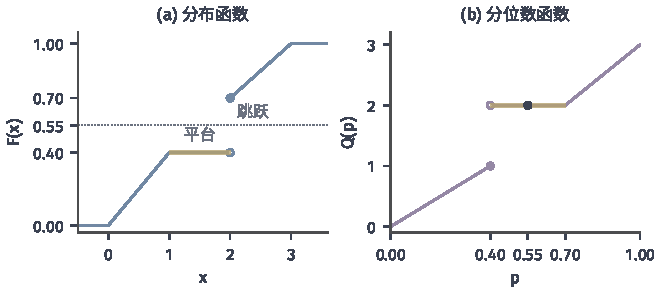
\includegraphics[width=112mm]{figures/01-basic-mathematics/05-probability-and-statistics-basics/matplotlib/prob-quantile-inverse/figure.pdf}
  \caption{分位数作为分布函数的广义逆。(a)分布函数在$[1,2)$上有平台（黄色），在$x=2$处从$0.4$跳到$0.7$；(b)相应的分位数函数$Q(p)=\inf\{x:F(x)\geq p\}$在$p=0.4$处从$1$跳到$2$，在$(0.4,0.7]$上保持为$2$（黄色）。点线$p=0.55$与(a)的曲线没有交点，(b)中黑点给出$Q(0.55)=2$。}
  \label{fig:prob-quantile-inverse}
\end{figure}

\begin{example}[几个分位数]
\label{ex:prob-quantile-examples}
例~\ref{ex:prob-three-cdfs}(b)中$F_T(t)=1-e^{-t}$连续严格递增，解$1-e^{-t}=p$得$Q(p)=-\ln(1-p)$。中位数是$\ln2\approx0.693$分钟，$0.9$分位数是$\ln10\approx2.303$分钟：九成顾客的等待不超过约$2.3$分钟。公平骰子的点数满足$F(3)=1/2$，所以中位数是$\inf\{x:F(x)\geq1/2\}=3$；尽管$[3,4)$上都有$F(x)=1/2$，约定取最小者$3$。
\end{example}

\paragraph{位置的不同度量}
均值、中位数和其他分位数都描述分布的“位置”，但回答的问题不同。中位数只依赖取值的顺序：它把概率分成各一半，与最大的那些值到底有多大无关。均值则按取值大小加权，远处的取值即使概率很小，也会把均值拉过去。分位数还可以描述其他位置，例如$0.9$分位数刻画右尾的典型界限，两个四分位数之差$Q(3/4)-Q(1/4)$则从另一个角度衡量离散程度。

若分布关于某点$c$对称且期望存在，则均值等于$c$，而$c$左右两侧的概率也各为一半，此时均值与中位数描述同一个中心；偏斜分布中二者通常不同。再引入\term{众数}（mode），即质量函数或密度函数取最大值的位置，它表示取值最集中的地方。

\begin{example}[右偏分布的三种位置]
\label{ex:prob-skewed-locations}
设$X$的密度为$f(x)=xe^{-x}$（$x>0$）。分部积分得$\int_0^\infty xe^{-x}\,\mathrm{d}x=1$，确为密度；均值$\mathbb{E}[X]=\int_0^\infty x^2e^{-x}\,\mathrm{d}x=2$。由$f'(x)=(1-x)e^{-x}$，众数为$1$。分布函数是$F(x)=1-(1+x)e^{-x}$，中位数$m$满足$(1+m)e^{-m}=1/2$，数值求解得$m\approx1.678$。三者满足众数$<$中位数$<$均值，如图~\ref{fig:prob-skewed-locations}所示：右侧的长尾把均值拉向右边，中位数受影响较小，众数只看密度峰的位置。
\end{example}

\begin{figure}[htbp]
  \centering
  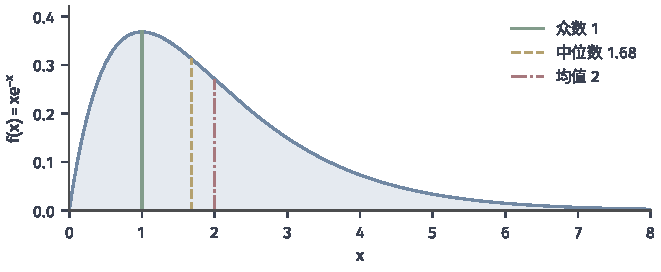
\includegraphics[width=112mm]{figures/01-basic-mathematics/05-probability-and-statistics-basics/matplotlib/prob-skewed-locations/figure.pdf}
  \caption{右偏密度$f(x)=xe^{-x}$（$x>0$）的三种位置。众数$1$是密度峰的位置，中位数约$1.68$把阴影面积分成相等的两半，均值$2$受右侧长尾影响最大。在这个右偏分布中，三者按众数、中位数、均值的顺序从左到右排列。}
  \label{fig:prob-skewed-locations}
\end{figure}

均值与中位数的差别在报告中很常见。收入、等待时间这类右偏变量，少数很大的取值会使均值明显高于中位数，此时“平均收入”与“典型收入”说的不是同一件事。选择哪种位置，取决于问题关心总量（均值乘以人数就是总量）还是典型个体（中位数）。

\subsection{矩、偏度与峰度}
\label{sec:prob-moments}

\paragraph{原点矩与中心矩}
均值与方差分别是$X$与$(X-\mu)^2$的期望。把幂次推广到一般正整数$k$，就得到一族数值特征，统称为矩。

\begin{definition}[矩]
\label{def:prob-moments}
设$k$为正整数且$\mathbb{E}\bigl[|X|^k\bigr]<\infty$。称$\mathbb{E}[X^k]$为$X$的$k$阶\term{原点矩}（raw moment），称$\mathbb{E}\bigl[(X-\mu)^k\bigr]$为$k$阶\term{中心矩}（central moment），其中$\mu=\mathbb{E}[X]$。
\end{definition}

在这个体系中，均值是一阶原点矩，方差是二阶中心矩；一阶中心矩恒为零。高阶矩有限是比低阶矩有限更强的要求：若$j<k$，由$|x|^j\leq1+|x|^k$，$k$阶矩有限蕴含$j$阶矩有限。中心矩可以用原点矩展开计算，例如$\mathbb{E}[(X-\mu)^3]=\mathbb{E}[X^3]-3\mu\,\mathbb{E}[X^2]+2\mu^3$。

尾部衰减的速度决定了哪些矩存在。设$X$的密度为$f(x)=3x^{-4}$（$x\geq1$）。则$\mathbb{E}[X]=\int_1^\infty3x^{-3}\,\mathrm{d}x=\frac32$，$\mathbb{E}[X^2]=\int_1^\infty3x^{-2}\,\mathrm{d}x=3$，方差为$3-\frac94=\frac34$；但$\mathbb{E}[X^3]=\int_1^\infty3x^{-1}\,\mathrm{d}x=+\infty$。这个分布有有限的均值和方差，三阶以上的矩都不存在。

\paragraph{偏度与峰度}
三阶、四阶中心矩记录了分布形状的信息，但它们随单位变化：把$X$乘以$a$，三阶中心矩乘以$a^3$。用标准差的相应次幂相除，就得到与单位无关的形状指标。

\begin{definition}[偏度与峰度]
\label{def:prob-skewness-kurtosis}
设$\operatorname{Var}(X)=\sigma^2>0$。若三阶矩有限，称$\gamma_1=\mathbb{E}\bigl[(X-\mu)^3\bigr]/\sigma^3$为$X$的\term{偏度}（skewness）；若四阶矩有限，称$\kappa=\mathbb{E}\bigl[(X-\mu)^4\bigr]/\sigma^4$为$X$的\term{峰度}（kurtosis）。
\end{definition}

偏度衡量不对称性：立方保留了偏差的符号，右侧远处的大偏差使偏度为正，左侧的使之为负；对称分布的偏度为零。峰度以四次方放大远离均值的偏差，主要反映尾部的厚重程度，而不是峰顶的尖锐。第~\ref{sec:prob-gaussian}节的高斯分布峰度为$3$，因此$\kappa-3$常称为超额峰度，用来与高斯尾部比较。

\begin{example}[等待时间的偏度与峰度]
\label{ex:prob-exponential-shape}
对密度$f(t)=e^{-t}$（$t\geq0$），分部积分递推给出$\int_0^\infty t^ke^{-t}\,\mathrm{d}t=k!$，即$\mathbb{E}[T^k]=k!$。于是$\mu=1$，$\sigma^2=2-1=1$，
\[
  \begin{aligned}
  \mathbb{E}[(T-1)^3]&=6-3\cdot2+3\cdot1-1=2,\\
  \mathbb{E}[(T-1)^4]&=24-4\cdot6+6\cdot2-4\cdot1+1=9 .
  \end{aligned}
\]
偏度为$2$，峰度为$9$：分布明显右偏，尾部比高斯分布厚得多。
\end{example}

有限个数值特征一般不能确定整个分布。以各$1/2$的概率取$\pm1$的变量与区间$(-\sqrt3,\sqrt3)$上的均匀分布，均值都是$0$、方差都是$1$、偏度都是$0$，前者只取两个值，后者却连续分布。即使所有阶的矩都存在且对应相等，两个分布也可能不同：第~\ref{sec:prob-density-change}节的对数正态分布就是经典例子，存在另一个分布与它的各阶矩全部相同。所以数值特征是对分布的概括，而不是替代；需要完整分布时，仍要回到分布函数、质量函数或密度。

\section{常见离散分布}
\label{sec:prob-discrete-models}

很多随机现象的分布可以由少数假设推出，并由一两个参数完全确定。本节按随机结果的含义组织离散模型：一次二元结果（Bernoulli分布）、一次类别选择（类别分布）、固定次数内的成功数（二项分布）、首次成功所需的次数（几何分布），以及没有固定上限的事件计数（Poisson分布）。每个模型都要说明它从什么假设得来，假设改变时为何不能沿用。图~\ref{fig:prob-discrete-pmfs}先给出后四类分布质量函数的样子。

\begin{figure*}[htbp]
  \centering
  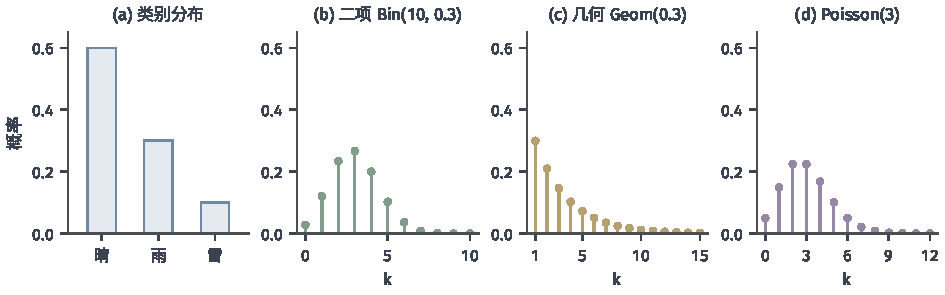
\includegraphics[width=160mm]{figures/01-basic-mathematics/05-probability-and-statistics-basics/matplotlib/prob-discrete-pmfs/figure.pdf}
  \caption{常见离散分布的质量函数。(a)三个天气类别的类别分布，概率依次为$0.6,0.3,0.1$，横轴只是类别标签；(b)$10$次独立试验、成功概率$0.3$的成功次数，集中在均值$3$附近；(c)成功概率$0.3$时首次成功所需的试验次数，从$1$开始按公比$0.7$递减；(d)均值为$3$的Poisson计数，取值没有上限，图中只画到$12$。}
  \label{fig:prob-discrete-pmfs}
\end{figure*}

\subsection{Bernoulli分布}
\label{sec:prob-bernoulli}

\paragraph{一次二元结果}
抽检一件产品是否为次品、一次点击是否发生、一枚硬币是否正面，都只有两种结果。把“成功”记为$1$、“失败”记为$0$，得到只取两个值的随机变量，它的分布只需一个参数。

\begin{definition}[Bernoulli分布]
\label{def:prob-bernoulli}
设$0\leq p\leq1$。若$\mathbb{P}(X=1)=p$，$\mathbb{P}(X=0)=1-p$，就称$X$服从参数为$p$的\term{Bernoulli分布}（Bernoulli distribution），记作$X\sim\operatorname{Bernoulli}(p)$。其质量函数可以统一写成
\[
  p_X(x)=p^x(1-p)^{1-x},\qquad x\in\{0,1\},
\]
其中约定$0^0=1$。
\end{definition}

直接计算$\mathbb{E}[X]=0\cdot(1-p)+1\cdot p=p$。由于$X$只取$0$和$1$，$X^2=X$，所以$\mathbb{E}[X^2]=p$，
\[
  \operatorname{Var}(X)=p-p^2=p(1-p).
\]
方差在$p=1/2$时最大，为$1/4$；$p$接近$0$或$1$时结果几乎确定，方差趋于零。

\paragraph{指示变量与事件概率}
任何事件$A$都对应一个Bernoulli变量，即它的指示变量$\mathbb{I}_A$，其参数就是$\mathbb{P}(A)$。于是
\[
  \mathbb{E}[\mathbb{I}_A]=\mathbb{P}(A).
\]
这个等式把概率写成了期望，从而可以借助期望的线性性计算“发生了几个事件”。设$A_1,\dots,A_n$为事件，$N=\mathbb{I}_{A_1}+\dots+\mathbb{I}_{A_n}$就是其中发生的个数，它的均值是$\mathbb{E}[N]=\sum_i\mathbb{P}(A_i)$。这里用到的是多个指示变量之和的线性性：$N$在每个样本点上都是各指示函数值之和，按样本点求概率加权和时可以逐项拆开（样本空间可数时这就是求和的线性性，一般情形见第~\ref{sec:rvec-moments}节）。这一步不需要任何独立性。

\begin{example}[抽检样本中次品个数的均值]
\label{ex:prob-inspection-mean}
回到例~\ref{ex:prob-inspection-hypergeometric}，从$5$件次品、$95$件合格品中不放回抽取$10$件。若按顺序抽取，第$i$件是哪一件产品，由对称性对$100$件产品等可能，所以“第$i$件是次品”的概率为$5/100$。样本中次品个数为$N=\sum_{i=1}^{10}\mathbb{I}_{A_i}$，其中$A_i$为“第$i$件是次品”，于是$\mathbb{E}[N]=10\times0.05=0.5$。各次抽取并不独立，但这不影响均值的计算。
\end{example}

同样，若$n$次试验中成功的指示变量为$X_1,\dots,X_n$，成功的比例$\frac1n\sum_iX_i$的均值等于各次成功概率的平均。频数、计数和样本比例都可以这样写成指示变量之和，后面各章会反复使用这一表示。

\subsection{类别分布}
\label{sec:prob-categorical}

\paragraph{有限个类别}
天气可以是晴、雨、雪，一张图片可以属于$K$个类别之一。把二元结果推广到有限个类别，就要为每个类别指定一个概率。

\begin{definition}[类别分布]
\label{def:prob-categorical}
设$\bm{\pi}=(\pi_1,\dots,\pi_K)^{\top}$满足$\pi_k\geq0$且$\sum_{k=1}^K\pi_k=1$。若随机变量$C$取值于$\{1,\dots,K\}$，且$\mathbb{P}(C=k)=\pi_k$，就称$C$服从\term{类别分布}（categorical distribution），记作$C\sim\operatorname{Cat}(\bm{\pi})$。
\end{definition}

满足上述条件的向量$\bm{\pi}$称为概率向量。$K=2$时，类别分布就是Bernoulli分布换了一种编号；公平骰子的点数是$K=6$、$\pi_k=1/6$的类别分布。图~\ref{fig:prob-discrete-pmfs}(a)画的是$\bm{\pi}=(0.6,0.3,0.1)^{\top}$的天气分布。

\paragraph{标签不是数量}
类别分布用$1,\dots,K$作编号，但这些数字只是标签，没有大小意义。若把晴、雨、雪编为$1,2,3$，“编号的均值”是$1\times0.6+2\times0.3+3\times0.1=1.5$；改为雪、雨、晴依次编$1,2,3$，同一个分布的“编号均值”就变成$3\times0.6+2\times0.3+1\times0.1=2.5$。结果随任意的编号方式而变，并不表示“平均天气介于晴和雨之间”。骰子点数是例外，因为点数本身就是数量。

需要对类别作数值计算时，常用独热编码（one-hot encoding）：把类别$C=k$表示成第$k$个分量为$1$、其余为$0$的向量$\bm{e}_C\in\mathbb{R}^K$。$\bm{e}_C$的第$k$个分量正是指示变量$\mathbb{I}_{\{C=k\}}$，其期望为$\pi_k$，所以$\bm{e}_C$的逐分量期望就是概率向量$\bm{\pi}$。这一表示不依赖编号顺序，向量值随机变量的系统讨论见第~\ref{chap:random-vectors}章。

\subsection{二项分布}
\label{sec:prob-binomial}

\paragraph{固定次数中的成功数}
把一次Bernoulli试验独立地重复$n$次，成功总次数是多少？例如有放回地抽检$10$件产品，每件是次品的概率为$0.05$，样本中的次品数就是这样的计数。设$X_1,\dots,X_n$为各次试验的成功指示，满足三个条件：试验次数$n$事先固定；每次成功概率都是$p$；各次试验相互独立，即事件$\{X_i=1\}$（$i=1,\dots,n$）相互独立。令$S=X_1+\dots+X_n$。

考虑$S=k$。任意一个指定位置有$k$次成功、$n-k$次失败的结果序列，由相互独立性，其概率是$p^k(1-p)^{n-k}$，与成功出现在哪些位置无关。从$n$个位置中选出$k$个成功位置共有$\binom nk$种方式（第~\ref{chap:counting}章），这些序列两两互斥，因此
\[
  \mathbb{P}(S=k)=\binom{n}{k}p^k(1-p)^{n-k},\qquad k=0,1,\dots,n .
\]

\begin{definition}[二项分布]
\label{def:prob-binomial}
具有上述质量函数的分布称为参数为$n,p$的\term{二项分布}（binomial distribution），记作$S\sim\operatorname{Bin}(n,p)$。
\end{definition}

由二项式定理，$\sum_{k=0}^n\binom nkp^k(1-p)^{n-k}=(p+1-p)^n=1$，质量函数确实归一。$n=1$时它就是$\operatorname{Bernoulli}(p)$。

\paragraph{均值与方差}
均值可以用指示变量之和直接得到：$\mathbb{E}[S]=\sum_i\mathbb{E}[X_i]=np$。方差要计算$\mathbb{E}[S^2]$，这里从质量函数出发。利用组合恒等式$k\binom nk=n\binom{n-1}{k-1}$及其推论$k(k-1)\binom nk=n(n-1)\binom{n-2}{k-2}$，
\[
  \begin{aligned}
  \mathbb{E}[S(S-1)]&=\sum_{k=2}^nn(n-1)\binom{n-2}{k-2}p^k(1-p)^{n-k}\\
  &=n(n-1)p^2\sum_{j=0}^{n-2}\binom{n-2}{j}p^j(1-p)^{n-2-j}=n(n-1)p^2,
  \end{aligned}
\]
最后一个和是$\operatorname{Bin}(n-2,p)$的总概率$1$。于是
\[
  \begin{aligned}
  \operatorname{Var}(S)&=\mathbb{E}[S(S-1)]+\mathbb{E}[S]-(\mathbb{E}[S])^2\\
  &=n(n-1)p^2+np-n^2p^2=np(1-p).
  \end{aligned}
\]
方差恰为$n$个Bernoulli方差之和；第~\ref{sec:rvec-moments}节会说明，这是独立变量的方差可以相加的一个特例。

\begin{example}[有放回抽检]
\label{ex:prob-inspection-binomial}
有放回地从次品率为$5\%$的产品中抽检$10$件，次品数$S\sim\operatorname{Bin}(10,0.05)$。样本中没有次品的概率是$0.95^{10}\approx0.5987$，均值为$0.5$，方差为$10\times0.05\times0.95=0.475$。
\end{example}

\paragraph{条件改变时}
二项模型的三个条件缺一不可。例~\ref{ex:prob-inspection-hypergeometric}是不放回抽检，每抽走一件，剩余产品的构成就变了，各次抽取不独立，样本中没有次品的概率是$0.5838$而不是$0.5987$。由于样本只占总体的$10\%$，两者相差不大；样本占总体比例越大，差别越明显。不放回抽样下次品数的精确分布称为超几何分布，其均值仍为$0.5$（例~\ref{ex:prob-inspection-mean}），方差则不同。

成功概率不相同时同样不能使用二项分布。设两次试验相互独立，第一次必然失败（$p_1=0$），第二次必然成功（$p_2=1$）。成功总数恒为$1$，方差为$0$；而平均成功概率为$1/2$的$\operatorname{Bin}(2,1/2)$方差为$1/2$。均值相同，波动却完全不同，原因是各次试验的概率并不一致。

\subsection{几何分布}
\label{sec:prob-geometric}

\paragraph{首次成功所需的次数}
反复掷骰子，直到第一次出现$6$点为止，要掷多少次？二项分布固定次数、数成功个数；这里反过来，次数本身是随机的。设各次试验相互独立、成功概率都是$p\in(0,1]$，令$T$为首次成功时已进行的试验次数。

$T=k$意味着前$k-1$次都失败、第$k$次成功，由独立性
\[
  \mathbb{P}(T=k)=(1-p)^{k-1}p,\qquad k=1,2,\dots
\]

\begin{definition}[几何分布]
\label{def:prob-geometric}
具有上述质量函数的分布称为参数为$p$的\term{几何分布}（geometric distribution），记作$T\sim\operatorname{Geom}(p)$。
\end{definition}

由几何级数，$\sum_{k\geq1}(1-p)^{k-1}p=p\cdot\frac{1}{1-(1-p)}=1$。“首次成功晚于第$k$次”等价于“前$k$次全部失败”，所以尾概率有简洁的形式
\[
  \mathbb{P}(T>k)=(1-p)^k,\qquad k=0,1,2,\dots
\]
掷骰子等待$6$点时$p=1/6$，掷了$6$次还没出现$6$点的概率是$(5/6)^6\approx0.335$，并不算小。

\paragraph{均值与方差}
对取非负整数值的变量，期望可以用尾概率求和：
\[
  \begin{aligned}
  \mathbb{E}[T]&=\sum_{k\geq1}k\,\mathbb{P}(T=k)=\sum_{k\geq1}\sum_{j=1}^{k}\mathbb{P}(T=k)\\
  &=\sum_{j\geq1}\sum_{k\geq j}\mathbb{P}(T=k)=\sum_{j\geq0}\mathbb{P}(T>j).
  \end{aligned}
\]
第三步交换了两个求和的次序，各项非负，交换不改变结果。代入尾概率得$\mathbb{E}[T]=\sum_{j\geq0}(1-p)^j=1/p$：成功概率为$1/6$时平均要掷$6$次。方差需要$\mathbb{E}[T(T-1)]$。记$q=1-p$，对几何级数$\sum_{k\geq0}q^k=\frac{1}{1-q}$在$|q|<1$内逐项求导两次（幂级数在收敛区间内可以逐项求导，见第~\ref{sec:ru-termwise-differentiation}节），得$\sum_{k\geq2}k(k-1)q^{k-2}=\frac{2}{(1-q)^3}$，于是
\[
  \begin{aligned}
  \mathbb{E}[T(T-1)]&=pq\sum_{k\geq2}k(k-1)q^{k-2}=\frac{2pq}{p^3}=\frac{2(1-p)}{p^2},\\
  \operatorname{Var}(T)&=\frac{2(1-p)}{p^2}+\frac1p-\frac1{p^2}=\frac{1-p}{p^2}.
  \end{aligned}
\]

\paragraph{无记忆性与计数约定}
已经连续失败了$m$次，还要再等多久？用条件概率计算：
\[
  \mathbb{P}(T>m+k\mid T>m)=\frac{\mathbb{P}(T>m+k)}{\mathbb{P}(T>m)}=\frac{(1-p)^{m+k}}{(1-p)^m}=(1-p)^k,
\]
它恰好等于$\mathbb{P}(T>k)$。这里用到$\{T>m+k\}\subseteq\{T>m\}$，所以交集就是$\{T>m+k\}$。结论称为\term{无记忆性}（memorylessness）：已经失败了多少次，不影响剩余等待次数的分布。这符合独立试验的设定，因为过去的失败不会让下一次更容易成功。“已经很久没出$6$点了，下一次该出了”的想法，在独立试验下并不成立。

文献中还有另一种约定：记录首次成功之前的失败次数$N=T-1$，取值于$\{0,1,2,\dots\}$，质量函数为$(1-p)^kp$。两者只相差一个平移，$\mathbb{E}[N]=\frac{1-p}{p}$比$\mathbb{E}[T]$小$1$，方差相同。使用几何分布的公式前，要先确认采用的是哪种计数。

\subsection{Poisson分布}
\label{sec:prob-poisson}

\paragraph{固定范围内的事件计数}
一小时内到达客服中心的电话数、一页书上的印刷错误数、一个像素在曝光时间内接收的光子数，都是在固定的时间、空间范围内对事件计数。与二项分布不同，这类计数没有预先固定的试验次数，原则上可以取任意非负整数。

\begin{definition}[Poisson分布]
\label{def:prob-poisson}
设$\lambda>0$。若$N$取非负整数值，且
\[
  \mathbb{P}(N=k)=e^{-\lambda}\frac{\lambda^k}{k!},\qquad k=0,1,2,\dots,
\]
就称$N$服从参数为$\lambda$的\term{Poisson分布}（Poisson distribution），记作$N\sim\operatorname{Poisson}(\lambda)$。
\end{definition}

由指数函数的幂级数$e^{\lambda}=\sum_{k\geq0}\lambda^k/k!$，质量函数之和为$1$。均值为
\[
  \mathbb{E}[N]=\sum_{k\geq1}k\,e^{-\lambda}\frac{\lambda^k}{k!}=\lambda e^{-\lambda}\sum_{k\geq1}\frac{\lambda^{k-1}}{(k-1)!}=\lambda .
\]
同样地，$\mathbb{E}[N(N-1)]=\lambda^2e^{-\lambda}\sum_{k\geq2}\frac{\lambda^{k-2}}{(k-2)!}=\lambda^2$，所以$\operatorname{Var}(N)=\lambda^2+\lambda-\lambda^2=\lambda$。参数$\lambda$同时是均值和方差。

\begin{example}[客服电话]
\label{ex:prob-poisson-calls}
设每小时来电数$N\sim\operatorname{Poisson}(3)$。一小时内没有来电的概率是$e^{-3}\approx0.0498$。来电不少于$5$个的概率为
\[
  1-e^{-3}\Bigl(1+3+\frac{9}{2}+\frac{27}{6}+\frac{81}{24}\Bigr)=1-16.375\,e^{-3}\approx0.185 .
\]
\end{example}

\paragraph{稀有事件的二项极限}
Poisson模型可以看作大量独立小机会的累计。把一小时切成$n$个小时段，假设每段至多来一个电话、来电概率为$\lambda/n$，且各段相互独立，那么来电总数服从$\operatorname{Bin}(n,\lambda/n)$，均值固定为$\lambda$。时段切得越细，这个二项分布越接近$\operatorname{Poisson}(\lambda)$。

\begin{theorem}[二项分布的Poisson极限]
\label{thm:prob-binomial-poisson-limit}
设$\lambda>0$，$p_n=\lambda/n$。对每个固定的非负整数$k$，
\[
  \lim_{n\to\infty}\binom{n}{k}p_n^k(1-p_n)^{n-k}=e^{-\lambda}\frac{\lambda^k}{k!}.
\]
\end{theorem}
\begin{proof}
把质量函数拆成三个因子：
\[
  \binom nk\Bigl(\frac\lambda n\Bigr)^k\Bigl(1-\frac\lambda n\Bigr)^{n-k}
  =\frac{\lambda^k}{k!}\cdot\frac{n(n-1)\cdots(n-k+1)}{n^k}\cdot\Bigl(1-\frac\lambda n\Bigr)^{n}\Bigl(1-\frac\lambda n\Bigr)^{-k}.
\]
$k$固定时，第二个因子是$k$个分别趋于$1$的因子$\frac{n-j}{n}$之积，极限为$1$；$(1-\lambda/n)^{-k}\to1$；而取对数后$n\ln(1-\lambda/n)\to-\lambda$，由指数函数的连续性$(1-\lambda/n)^n\to e^{-\lambda}$，这与第~\ref{chap:univariate-differentiation}章处理$(1+1/n)^n\to e$的方法相同。三者相乘即得结论。
\end{proof}

图~\ref{fig:prob-binomial-poisson}比较了$\operatorname{Bin}(n,3/n)$与$\operatorname{Poisson}(3)$。$n=6$时二项分布明显更集中于均值附近，因为它最多只能取到$6$；$n=60$时两者在图上几乎重合。这也说明了两个模型的差别：二项计数有已知的上限$n$，方差$np(1-p)$小于均值；Poisson计数没有上限，方差等于均值。只因均值接近就混用两个模型是不对的，要看计数是否有固定的试验次数，以及每次机会是否稀少。

\begin{figure}[htbp]
  \centering
  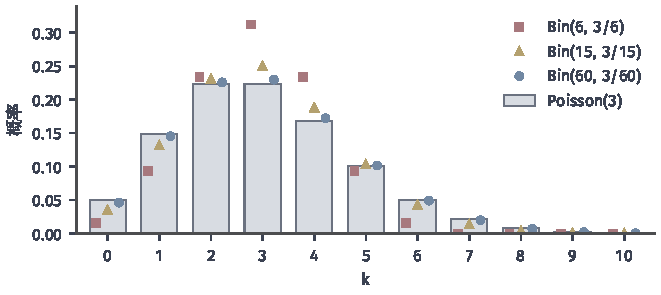
\includegraphics[width=112mm]{figures/01-basic-mathematics/05-probability-and-statistics-basics/matplotlib/prob-binomial-poisson/figure.pdf}
  \caption{稀有事件下二项分布逼近Poisson分布。灰色柱为$\operatorname{Poisson}(3)$的质量函数，三种标记分别为$n=6,15,60$、成功概率$3/n$的二项分布，均值都为$3$。$n$越大，二项分布越接近灰色柱；$n=6$时二项分布在$k=3$处偏高，并且不能取大于$6$的值。}
  \label{fig:prob-binomial-poisson}
\end{figure}

定理只说明了一种来源：满足“机会很多、每次很稀少、彼此独立”时，Poisson模型是合理的近似。仅知道计数非负并不足以采用Poisson分布；例如若来电成批出现，方差会明显大于均值。不同时间段的计数之间怎样联系、到达时刻怎样分布，需要Poisson过程来描述，可参考\BookChapterRef{chap:random-sequences-and-processes}{卷3《数学准备：优化、动力系统与信号处理》的“随机序列与随机过程”章}。

\section{常见连续分布}
\label{sec:prob-continuous-models}

连续模型同样从取值范围和形状假设出发。本节依次研究：有界区间上不偏向任何位置的取值（均匀分布），非负的等待时间（指数分布），围绕中心对称波动的量（高斯分布），以及更一般的正值变量与比例（Gamma分布与Beta分布）。图~\ref{fig:prob-continuous-densities}汇总了后四类分布在不同参数下的密度。

\begin{figure*}[htbp]
  \centering
  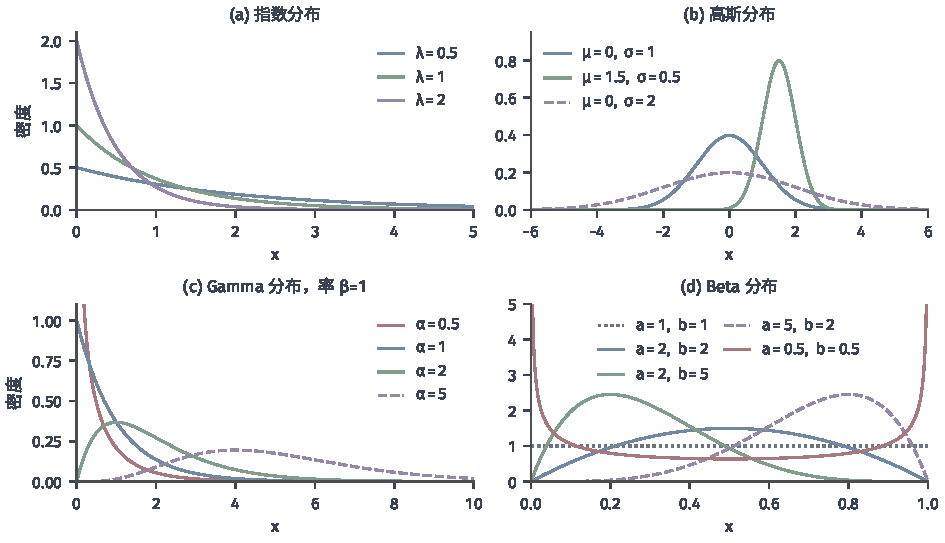
\includegraphics[width=160mm]{figures/01-basic-mathematics/05-probability-and-statistics-basics/matplotlib/prob-continuous-densities/figure.pdf}
  \caption{常见连续分布的密度。(a)指数分布，率$\lambda$越大，密度在$0$处越高、衰减越快；(b)高斯分布，$\mu$决定中心，$\sigma$决定宽度，$\sigma$减半时峰高加倍；(c)率为$1$的Gamma分布，形状$\alpha<1$时密度在$0$附近无界（图中截断），$\alpha=1$即指数分布，$\alpha>1$时出现单峰；(d)Beta分布，$a=b=1$为均匀分布，$a=b>1$关于$1/2$对称，$a<b$时偏向$0$、$a>b$时偏向$1$，$a=b=0.5$时呈U形（图中截断）。}
  \label{fig:prob-continuous-densities}
\end{figure*}

\subsection{均匀分布}
\label{sec:prob-uniform}

\paragraph{等长区间等概率}
把一根长为$1$米的绳子随机剪断，若没有理由认为任何位置更容易被剪中，自然要求长度相同的两段区间被剪中的概率相同。这一要求决定了密度在区间内必须是常数。

\begin{definition}[均匀分布]
\label{def:prob-uniform}
设$a<b$。若$X$的密度为
\[
  f_X(x)=\frac{1}{b-a},\qquad a<x<b,
\]
在区间外为$0$，就称$X$服从区间$(a,b)$上的\term{均匀分布}（uniform distribution），记作$X\sim\operatorname{U}(a,b)$。
\end{definition}

对$a\leq x\leq b$，分布函数为$F_X(x)=\frac{x-a}{b-a}$，在$x<a$时为$0$、$x>b$时为$1$。由对称性或直接积分，$\mathbb{E}[X]=\frac{a+b}{2}$。再由$\mathbb{E}[X^2]=\frac{1}{b-a}\int_a^bx^2\,\mathrm{d}x=\frac{a^2+ab+b^2}{3}$，
\[
  \operatorname{Var}(X)=\frac{a^2+ab+b^2}{3}-\frac{(a+b)^2}{4}=\frac{(b-a)^2}{12}.
\]
标准差$\frac{b-a}{2\sqrt3}\approx0.29(b-a)$与区间长度成正比，与区间位置无关。

\paragraph{均匀的含义与用途}
区间内密度相同，意思是任何子区间的概率只取决于它的长度：$\mathbb{P}(c<X\leq d)=\frac{d-c}{b-a}$，与子区间在哪里无关。这是一个关于对称性的模型假设，并不等于“对结果一无所知”。例如对一个正数比例$R$，若假设$R$在$(0,1)$上均匀，那么$R^2$就不再均匀（第~\ref{sec:prob-cdf-method}节的方法可以算出它的分布）；对同一未知量的不同表示，“均匀”给出不同的结论。

标准均匀变量$U\sim\operatorname{U}(0,1)$是随机模拟的基础。计算机的随机数生成器产生近似服从$\operatorname{U}(0,1)$的数，其他分布的随机数则由它经过变换得到。第~\ref{sec:prob-cdf-method}节会给出第一个例子：$U$经过对数变换后服从指数分布；一般的构造留到第~\ref{sec:rvec-generation}节。

\subsection{指数分布}
\label{sec:prob-exponential}

\paragraph{等待时间模型}
例~\ref{ex:prob-three-cdfs}(b)的等待时间满足$\mathbb{P}(T>t)=e^{-t}$。允许不同的时间尺度，就得到一族非负等待时间模型，用率参数$\lambda$表示单位时间内事件发生的强度。

\begin{definition}[指数分布]
\label{def:prob-exponential}
设$\lambda>0$。若$T$的密度为
\[
  f_T(t)=\lambda e^{-\lambda t},\qquad t\geq0,
\]
在$t<0$时为$0$，就称$T$服从率为$\lambda$的\term{指数分布}（exponential distribution），记作$T\sim\operatorname{Exp}(\lambda)$。
\end{definition}

积分得分布函数$F_T(t)=1-e^{-\lambda t}$与尾概率$\mathbb{P}(T>t)=e^{-\lambda t}$（$t\geq0$）。换元$s=\lambda t$并利用$\int_0^\infty s^ke^{-s}\,\mathrm{d}s=k!$（例~\ref{ex:prob-exponential-shape}），得$\mathbb{E}[T^k]=k!/\lambda^k$，于是
\[
  \mathbb{E}[T]=\frac1\lambda,\qquad \operatorname{Var}(T)=\frac{2}{\lambda^2}-\frac1{\lambda^2}=\frac1{\lambda^2}.
\]
率$\lambda$越大，事件来得越快，平均等待$1/\lambda$越短。标准差与均值相等。

\begin{example}[窗口等待]
\label{ex:prob-exponential-wait}
设等待时间平均为$5$分钟，取$T\sim\operatorname{Exp}(0.2)$。等待超过$10$分钟的概率是$e^{-2}\approx0.135$。中位数$\frac{\ln2}{0.2}\approx3.47$分钟，小于均值$5$分钟，这与第~\ref{sec:prob-quantiles}节右偏分布的规律一致；$0.9$分位数为$5\ln10\approx11.5$分钟。
\end{example}

\paragraph{无记忆性}
指数分布与几何分布一样具有无记忆性：对$s,t\geq0$，
\[
  \mathbb{P}(T>s+t\mid T>s)=\frac{\mathbb{P}(T>s+t)}{\mathbb{P}(T>s)}=\frac{e^{-\lambda(s+t)}}{e^{-\lambda s}}=e^{-\lambda t}=\mathbb{P}(T>t).
\]
已经等了$s$分钟，剩余等待时间超过$t$的概率与刚开始等时完全相同。

这种相似并非巧合，指数分布可以看作几何分布的连续时间版本。把时间切成长度为$h$的小段，每段内事件发生的概率为$\lambda h$，各段独立，首次发生所在的段数$T_h\sim\operatorname{Geom}(\lambda h)$。对应的等待时间约为$hT_h$，其尾概率$\mathbb{P}(hT_h>t)=(1-\lambda h)^{\lfloor t/h\rfloor}$在$h\to0$时趋于$e^{-\lambda t}$。几何分布数的是离散的试验次数，指数分布量的是连续的时间长度，二者的无记忆性都来自“每一刻发生的机会不随已等待的时间改变”。

无记忆性不是所有等待时间都有的性质。若等待时间$T\sim\operatorname{U}(0,10)$，已知已等了$5$分钟，再等超过$2$分钟的概率是$\mathbb{P}(T>7\mid T>5)=\frac{3/10}{5/10}=0.6$，而一开始等待超过$2$分钟的概率是$0.8$：等得越久，剩余的等待越短。机械零件因磨损而老化，其寿命也不满足无记忆性。是否采用指数模型，要看“剩余等待与已等待时间无关”这一假设是否合理。

\subsection{高斯分布}
\label{sec:prob-gaussian}

\paragraph{标准高斯密度}
测量误差、身高、考试成绩这类量，常在一个中心值两侧对称波动，离中心越远越少见。描述这种形状最重要的模型是高斯分布，也称正态分布。我们先看中心在$0$、尺度为$1$的情形。

\begin{definition}[高斯分布]
\label{def:prob-gaussian}
密度
\[
  \varphi(z)=\frac{1}{\sqrt{2\pi}}e^{-z^2/2},\qquad z\in\mathbb{R}
\]
称为标准高斯密度，具有该密度的$Z$称为服从\term{标准正态分布}（standard normal distribution），记作$Z\sim\mathcal{N}(0,1)$。设$\mu\in\mathbb{R}$，$\sigma>0$，若$X$的密度为
\[
  f_X(x)=\frac{1}{\sqrt{2\pi}\,\sigma}\exp\Bigl(-\frac{(x-\mu)^2}{2\sigma^2}\Bigr)=\frac1\sigma\varphi\Bigl(\frac{x-\mu}{\sigma}\Bigr),
\]
就称$X$服从参数为$\mu,\sigma^2$的\term{高斯分布}（Gaussian distribution），也称\term{正态分布}（normal distribution），记作$X\sim\mathcal{N}(\mu,\sigma^2)$。
\end{definition}

$\varphi$的归一化依赖积分$\int_{-\infty}^{\infty}e^{-z^2/2}\,\mathrm{d}z=\sqrt{2\pi}$。$e^{-z^2/2}$没有初等原函数，这个积分值通常借助二重积分的极坐标换元求得（第~\ref{chap:multivariate-integration}章）。$\varphi$是偶函数，且尾部比任何多项式衰减得都快，所以各阶矩都有限，奇函数$z\varphi(z)$的积分为零，$\mathbb{E}[Z]=0$。方差由分部积分得到：利用$\varphi'(z)=-z\varphi(z)$，
\[
  \mathbb{E}[Z^2]=\int_{-\infty}^{\infty}z\cdot z\varphi(z)\,\mathrm{d}z=\Bigl[-z\varphi(z)\Bigr]_{-\infty}^{\infty}+\int_{-\infty}^{\infty}\varphi(z)\,\mathrm{d}z=1 .
\]
所以$\operatorname{Var}(Z)=1$。同样分部积分一次可得$\mathbb{E}[Z^4]=3\,\mathbb{E}[Z^2]=3$，这就是第~\ref{sec:prob-moments}节所说高斯分布的峰度为$3$。一般的$X\sim\mathcal{N}(\mu,\sigma^2)$由$Z$平移缩放而来（第~\ref{sec:prob-standardization}节），因此$\mathbb{E}[X]=\mu$，$\operatorname{Var}(X)=\sigma^2$：两个参数正好是均值与方差。图~\ref{fig:prob-continuous-densities}(b)显示，$\mu$平移曲线的中心，$\sigma$同时决定宽度与峰高，$\sigma$越小，曲线越窄越高，面积始终为$1$。

\paragraph{尾概率}
标准正态的分布函数记作$\Phi(z)=\int_{-\infty}^z\varphi(t)\,\mathrm{d}t$。它没有初等表达式，需要查表或用软件计算。对称性给出$\Phi(-z)=1-\Phi(z)$，常用的几个值是
\[
  \mathbb{P}(|Z|\leq1)\approx0.683,\qquad \mathbb{P}(|Z|\leq2)\approx0.954,\qquad \mathbb{P}(|Z|\leq3)\approx0.997 .
\]
偏离均值超过三个标准差的概率不到$0.3\%$。高斯尾部衰减得极快，对$z>0$有估计
\[
  \mathbb{P}(Z>z)=\int_z^\infty\varphi(t)\,\mathrm{d}t\leq\int_z^\infty\frac tz\varphi(t)\,\mathrm{d}t=\frac{\varphi(z)}{z},
\]
其中不等号用到积分区域内$t/z\geq1$，最后一步利用$t\varphi(t)$的原函数是$-\varphi(t)$。尾概率至少以$e^{-z^2/2}$的速度下降，比指数分布的$e^{-\lambda t}$快得多。

\paragraph{标准化计算与分位数}
对一般的$X\sim\mathcal{N}(\mu,\sigma^2)$，在概率积分中换元$z=(x-\mu)/\sigma$，$\mathrm{d}x=\sigma\,\mathrm{d}z$，得
\[
  \begin{aligned}
  \mathbb{P}(a<X\leq b)&=\int_a^b\frac1\sigma\varphi\Bigl(\frac{x-\mu}{\sigma}\Bigr)\mathrm{d}x=\int_{(a-\mu)/\sigma}^{(b-\mu)/\sigma}\varphi(z)\,\mathrm{d}z\\
  &=\Phi\Bigl(\frac{b-\mu}{\sigma}\Bigr)-\Phi\Bigl(\frac{a-\mu}{\sigma}\Bigr).
  \end{aligned}
\]
所以任何高斯分布的概率都可以化为标准正态的分布函数值，只需一张$\Phi$的表。反方向，记标准正态的$p$分位数为$z_p=\Phi^{-1}(p)$，则$\mathcal{N}(\mu,\sigma^2)$的$p$分位数是$\mu+\sigma z_p$。常用值有$z_{0.95}\approx1.645$、$z_{0.975}\approx1.960$、$z_{0.99}\approx2.326$；由对称性$z_{1-p}=-z_p$。

\begin{example}[零件长度]
\label{ex:prob-gaussian-parts}
某零件长度$X\sim\mathcal{N}(50,0.2^2)$，单位为毫米，合格范围为$[49.6,50.4]$。标准化后，合格概率为$\Phi(2)-\Phi(-2)\approx0.954$。若要找一个上限，使只有$1\%$的零件超过它，则取$0.99$分位数$50+0.2\times2.326\approx50.47$毫米。
\end{example}

高斯分布在应用中如此常见，一个重要原因是许多独立小误差之和近似服从高斯分布。这需要对“和”的分布作专门研究，具体条件和含义见第~\ref{sec:samp-clt}节的中心极限定理；仅凭“误差是对称的”并不能推出高斯形状。

\subsection{Gamma分布}
\label{sec:prob-gamma}

\paragraph{Gamma函数与归一化}
例~\ref{ex:prob-skewed-locations}的密度$xe^{-x}$与指数密度$e^{-x}$都具有$x^{\alpha-1}e^{-\beta x}$的形状。它们构成一族灵活的正值分布：幂函数因子控制$0$附近的行为，指数因子控制尾部。要使这个形状成为密度，需要计算它的积分，这就引出Gamma函数。

\begin{definition}[Gamma函数]
\label{def:prob-gamma-function}
对$\alpha>0$，定义\term{Gamma函数}（Gamma function）
\[
  \Gamma(\alpha)=\int_0^\infty t^{\alpha-1}e^{-t}\,\mathrm{d}t .
\]
\end{definition}

条件$\alpha>0$保证$t^{\alpha-1}$在$0$附近可积，$e^{-t}$保证无穷远处可积，两处的反常积分都收敛（第~\ref{sec:ru-improper-integrals}节）。分部积分给出递推
\[
  \Gamma(\alpha+1)=\Bigl[-t^{\alpha}e^{-t}\Bigr]_0^\infty+\alpha\int_0^\infty t^{\alpha-1}e^{-t}\,\mathrm{d}t=\alpha\,\Gamma(\alpha),
\]
又$\Gamma(1)=1$，所以对正整数$n$有$\Gamma(n)=(n-1)!$，Gamma函数把阶乘延伸到正实数。换元$t=z^2/2$还给出$\Gamma(1/2)=\sqrt{2}\int_0^\infty e^{-z^2/2}\,\mathrm{d}z=\sqrt\pi$。对$\beta>0$，再换元$t=\beta x$，
\[
  \int_0^\infty x^{\alpha-1}e^{-\beta x}\,\mathrm{d}x=\frac{\Gamma(\alpha)}{\beta^\alpha}.
\]

\begin{definition}[Gamma分布]
\label{def:prob-gamma}
设$\alpha>0$，$\beta>0$。若$X$的密度为
\[
  f_X(x)=\frac{\beta^\alpha}{\Gamma(\alpha)}x^{\alpha-1}e^{-\beta x},\qquad x>0,
\]
在$x\leq0$时为$0$，就称$X$服从形状参数为$\alpha$、率参数为$\beta$的\term{Gamma分布}（Gamma distribution），记作$X\sim\operatorname{Gamma}(\alpha,\beta)$。
\end{definition}

由上式，密度的积分为$1$。同一个积分公式直接给出各阶矩：
\[
  \mathbb{E}[X^k]=\frac{\beta^\alpha}{\Gamma(\alpha)}\int_0^\infty x^{\alpha+k-1}e^{-\beta x}\,\mathrm{d}x=\frac{\Gamma(\alpha+k)}{\Gamma(\alpha)\beta^k}.
\]
由递推，$\mathbb{E}[X]=\alpha/\beta$，$\mathbb{E}[X^2]=\alpha(\alpha+1)/\beta^2$，于是$\operatorname{Var}(X)=\alpha/\beta^2$。形状参数决定曲线的样子：$\alpha<1$时密度在$0$附近趋于无穷；$\alpha=1$时在$0$处取最大值；$\alpha>1$时密度从$0$升起再下降，由导数为零得众数$(\alpha-1)/\beta$。图~\ref{fig:prob-continuous-densities}(c)画出了这三种情形。

\paragraph{特例与参数化}
$\alpha=1$时密度为$\beta e^{-\beta x}$，所以$\operatorname{Exp}(\lambda)=\operatorname{Gamma}(1,\lambda)$；例~\ref{ex:prob-skewed-locations}的密度$xe^{-x}$就是$\operatorname{Gamma}(2,1)$，其均值$2$、众数$1$与前面的计算一致。第~\ref{sec:rvec-transforms}节将证明，$n$个相互独立的$\operatorname{Exp}(\lambda)$等待时间之和服从$\operatorname{Gamma}(n,\lambda)$，这给出了整数形状参数的含义：等到第$n$个事件发生所需的总时间。

Gamma分布有两种常见的参数化。本书使用率参数$\beta$，它的单位是“每单位时间”；另一种使用尺度参数$\vartheta=1/\beta$，密度写作$\frac{1}{\Gamma(\alpha)\vartheta^\alpha}x^{\alpha-1}e^{-x/\vartheta}$，均值为$\alpha\vartheta$。两种写法描述同一族分布，但同一组数字含义不同：把“$\operatorname{Gamma}(2,0.5)$”读作率参数，均值是$2/0.5=4$；读作尺度参数，均值是$2\times0.5=1$。查阅公式或调用软件时，必须先确认用的是哪一种。

\subsection{Beta分布}
\label{sec:prob-beta}

\paragraph{区间上的比例}
点击率、合格率、某种成分的比例都在$0$与$1$之间。均匀分布对这类量太死板，我们希望有一族在$(0,1)$上形状灵活的分布，能偏向$0$、偏向$1$或集中在中间。仿照Gamma分布，取$r^{a-1}(1-r)^{b-1}$的形状，两个幂次分别控制两端附近的行为。

\begin{definition}[Beta分布]
\label{def:prob-beta}
对$a>0$，$b>0$，记\term{Beta函数}（Beta function）
\[
  B(a,b)=\int_0^1r^{a-1}(1-r)^{b-1}\,\mathrm{d}r .
\]
若$R$的密度为
\[
  f_R(r)=\frac{1}{B(a,b)}r^{a-1}(1-r)^{b-1},\qquad 0<r<1,
\]
在区间外为$0$，就称$R$服从参数为$a,b$的\term{Beta分布}（Beta distribution），记作$R\sim\operatorname{Beta}(a,b)$。
\end{definition}

$a,b>0$保证两端的反常积分收敛。$a=b=1$时密度恒为$1$，就是$\operatorname{U}(0,1)$。$a=b>1$时密度关于$1/2$对称、中间高两端低；$a>b$时概率偏向$1$，$a<b$时偏向$0$；$a,b<1$时密度在两端趋于无穷，呈U形。见图~\ref{fig:prob-continuous-densities}(d)。

\paragraph{均值与方差}
矩的计算归结为Beta函数之比：$\mathbb{E}[R]=B(a+1,b)/B(a,b)$。为求这个比值，先注意$r^{a-1}(1-r)^{b-1}=r^{a}(1-r)^{b-1}+r^{a-1}(1-r)^{b}$（把$1=r+(1-r)$乘进去），积分得
\[
  B(a,b)=B(a+1,b)+B(a,b+1).
\]
另一方面，对$B(a+1,b)=\int_0^1r^a(1-r)^{b-1}\,\mathrm{d}r$分部积分，取$-\frac1b(1-r)^b$为$(1-r)^{b-1}$的原函数，边界项在两端为零，得$B(a+1,b)=\frac abB(a,b+1)$。把两式联立消去$B(a,b+1)$，
\[
  B(a+1,b)=\frac{a}{a+b}B(a,b),\qquad\text{从而}\qquad\mathbb{E}[R]=\frac{a}{a+b}.
\]
再用一次同样的递推，$\mathbb{E}[R^2]=\frac{B(a+2,b)}{B(a,b)}=\frac{a+1}{a+b+1}\cdot\frac{a}{a+b}$，于是
\[
  \operatorname{Var}(R)=\frac{a(a+1)}{(a+b)(a+b+1)}-\frac{a^2}{(a+b)^2}=\frac{ab}{(a+b)^2(a+b+1)}.
\]
均值只取决于$a$在$a+b$中的比例，而$a+b$越大方差越小，分布越集中。例如$\operatorname{Beta}(2,8)$与$\operatorname{Beta}(20,80)$的均值都是$0.2$，方差分别约为$0.0145$与$0.0016$。

\paragraph{用途与构造}
Beta分布常用来描述一个随机比例，或者表达对未知成功概率$p$的不确定性：$a$、$b$可以理解为“相当于事先见过的成功与失败次数”，$a+b$越大，对$p$的判断越确定。第~\ref{sec:est-bayes}节会用它作为二项模型中成功概率的先验分布。Beta函数还与Gamma函数有关系$B(a,b)=\Gamma(a)\Gamma(b)/\Gamma(a+b)$，它来自一个构造：两个相互独立、率相同的Gamma变量$U\sim\operatorname{Gamma}(a,1)$、$V\sim\operatorname{Gamma}(b,1)$，比例$U/(U+V)$服从$\operatorname{Beta}(a,b)$。证明需要二元变量的变换，留到第~\ref{sec:rvec-transforms}节。

\section{一元随机变量的变换}
\label{sec:prob-univariate-transforms}
\label{sec:rv-pushforward}

知道等待时间$T$的分布，费用$2T+5$元、等待时间的对数$\ln T$、误差的平方$\varepsilon^2$的分布是什么？本节研究$Y=g(X)$的分布怎样由$X$的分布和函数$g$确定。我们先用分布函数给出对任何分布都适用的方法，再在可微条件下推出密度的变换公式，最后专门讨论最常用的平移、缩放与标准化。

\subsection{利用分布函数计算变换}
\label{sec:prob-cdf-method}

\paragraph{回到原变量的事件}
$Y=g(X)$仍是定义在同一样本空间上的随机变量，对每个结果$\omega$，$Y(\omega)=g(X(\omega))$。要求$Y$的分布函数，就把事件$\{Y\leq y\}$翻译回$X$的取值范围：
\[
  F_Y(y)=\mathbb{P}(g(X)\leq y)=\mathbb{P}\bigl(X\in\{x:g(x)\leq y\}\bigr).
\]
一般地，对实数集的子集$B$，有$\mathbb{P}(Y\in B)=\mathbb{P}\bigl(X\in g^{-1}(B)\bigr)$，其中$g^{-1}(B)=\{x:g(x)\in B\}$是$B$的逆像。由此得到的$Y$的分布，也称为$X$的分布经$g$的\term{分布推前}（pushforward），记作$P_{g(X)}$或$g_{\#}P_X$，即$g_{\#}P_X(B)=P_X\bigl(g^{-1}(B)\bigr)$。

实际计算分两步。先确定$Y$可能取值的范围，即$g$在$X$可能取值上的像；在这个范围之外，分布函数直接是$0$或$1$。再对范围内的每个$y$，解出不等式$g(x)\leq y$对应的$x$的集合，用$X$的分布计算它的概率。

\begin{example}[由均匀变量得到指数变量]
\label{ex:prob-uniform-to-exponential}
设$U\sim\operatorname{U}(0,1)$，$\lambda>0$，令$Y=-\frac1\lambda\ln(1-U)$。$1-U$取值于$(0,1)$，其对数为负，所以$Y$取值于$(0,\infty)$，$y\leq0$时$F_Y(y)=0$。对$y>0$，由于$u\mapsto-\frac1\lambda\ln(1-u)$严格递增，
\[
  F_Y(y)=\mathbb{P}\Bigl(-\tfrac1\lambda\ln(1-U)\leq y\Bigr)=\mathbb{P}\bigl(U\leq1-e^{-\lambda y}\bigr)=1-e^{-\lambda y}.
\]
这正是$\operatorname{Exp}(\lambda)$的分布函数。这个例子说明了随机模拟中怎样把均匀随机数变成指数随机数：所用的函数恰是指数分布函数的反函数。
\end{example}

\paragraph{非单调变换}
单调函数把$\{g(x)\leq y\}$变成一个区间，计算很直接。非单调时，一个$y$值可能来自多个$x$值，逆像可能是几段区间的并。最典型的是平方：对$y\geq0$，
\[
  \{X^2\leq y\}=\{-\sqrt y\leq X\leq\sqrt y\},\qquad
  F_{X^2}(y)=F_X(\sqrt y)-F_X\bigl((-\sqrt y)^-\bigr),
\]
$y<0$时$F_{X^2}(y)=0$。左端点用左极限，是因为区间包含$-\sqrt y$。这个公式对任何分布都成立，不要求$X$有密度。

\begin{example}[离散变量的平方]
\label{ex:prob-discrete-square}
设$X$在$\{-1,0,1,2\}$上等可能取值。$Y=X^2$的可能取值为$0,1,4$。$Y=1$的逆像是$\{-1,1\}$两个点，所以
\[
  \mathbb{P}(Y=0)=\frac14,\qquad\mathbb{P}(Y=1)=\frac14+\frac14=\frac12,\qquad\mathbb{P}(Y=4)=\frac14 .
\]
平方把$-1$与$1$合并到同一个值，它们的概率相加。
\end{example}

图~\ref{fig:prob-square-transform}(a)画出$X\sim\operatorname{U}(-1,2)$时的情形。阈值$y=0.49<1$时，逆像是对称的区间$[-0.7,0.7]$，两侧都在$X$的取值范围内；阈值$y=2.25>1$时，$-\sqrt y=-1.5$已在取值范围之外，逆像只剩$[-1,1.5]$。于是对$0\leq y\leq1$有$F_Y(y)=\frac{2\sqrt y}{3}$，对$1\leq y\leq4$有$F_Y(y)=\frac{\sqrt y+1}{3}$。同一个函数$g$，在$Y$取值范围的不同部分，逆像的形状也可能不同。

\subsection{密度的变量替换}
\label{sec:prob-density-change}

\paragraph{单调变换的密度公式}
若$X$有密度，我们常希望直接写出$Y$的密度，而不是每次都先求分布函数。在$g$严格单调且可微的条件下，从分布函数出发就能得到一个通用公式。

\begin{theorem}[一元密度的变量替换]
\label{thm:prob-density-change}
设$X$有密度$f_X$，且$f_X$在开区间$I$外为零。设$g:I\to J$是从$I$到开区间$J$的连续可微双射，且在$I$上$g'(x)\neq0$，其反函数记为$h=g^{-1}:J\to I$。则$Y=g(X)$有密度
\[
  f_Y(y)=f_X\bigl(h(y)\bigr)\,\bigl|h'(y)\bigr|,\qquad y\in J,
\]
在$J$外为零。
\end{theorem}
\begin{proof}
$g'$在区间$I$上连续且不为零，所以$g'$不变号，$g$严格单调，$h$也连续可微，且$h'(y)=1/g'(h(y))$。设$g$递增，并记$J=(c,d)$、$I=(a',b')$（端点可以是无穷）。对$y\in J$，$g(X)\leq y$等价于$X\leq h(y)$，于是
\[
  F_Y(y)=\int_{a'}^{h(y)}f_X(x)\,\mathrm{d}x=\int_{c}^{y}f_X\bigl(h(s)\bigr)h'(s)\,\mathrm{d}s,
\]
第二步是换元$x=h(s)$（定理~\ref{thm:ru-substitution}，在反常积分上取极限即可）。这说明$Y$的分布函数是$f_X(h(s))h'(s)$的累计，而$h'>0$，所以它就是$Y$的密度。若$g$递减，则$g(X)\leq y$等价于$X\geq h(y)$，同样换元得$F_Y(y)=\int_c^yf_X(h(s))\,(-h'(s))\,\mathrm{d}s$，此时$-h'(s)=|h'(s)|$。

若$f_X$在$h(y)$处连续，也可以直接对$F_Y(y)=F_X(h(y))$（递增情形）求导：由链式法则，$F_Y'(y)=f_X(h(y))\,h'(y)$，结果相同。上面用换元写出积分，是为了不必假设$f_X$连续。
\end{proof}

绝对导数因子$|h'(y)|$补偿的是区间长度的伸缩。$X$落在$x$附近长为$\Delta x$的小区间内的概率约为$f_X(x)\Delta x$，这个小区间被$g$映到$y=g(x)$附近长为$\Delta y\approx|g'(x)|\Delta x$的小区间，概率不变，于是$f_Y(y)\Delta y\approx f_X(x)\Delta x$，即$f_Y(y)\approx f_X(x)/|g'(x)|=f_X(h(y))|h'(y)|$。$g$把区间拉长的地方，密度相应降低；压缩的地方，密度相应升高。只把$x=h(y)$代入$f_X$而遗漏这个因子，所得函数一般积分不为$1$。

\begin{example}[对数正态分布]
\label{ex:prob-lognormal}
设$X\sim\mathcal{N}(\mu,\sigma^2)$，$Y=e^X$。这里$I=\mathbb{R}$，$J=(0,\infty)$，$h(y)=\ln y$，$h'(y)=1/y$。由定理~\ref{thm:prob-density-change}，
\[
  f_Y(y)=\frac{1}{\sigma y}\varphi\Bigl(\frac{\ln y-\mu}{\sigma}\Bigr),\qquad y>0 .
\]
$Y$称为服从对数正态分布，它是一个右偏的正值分布，常用于收入、粒径等乘性变化的量。因子$1/y$来自指数函数在$y$较大处把区间大幅拉长。
\end{example}

变量替换也补全了定理~\ref{thm:prob-lotus}中密度情形的一部分。在定理~\ref{thm:prob-density-change}的条件下，按$Y$的密度计算期望，再换元$y=g(x)$：
\[
  \mathbb{E}[Y]=\int_Jy\,f_X\bigl(h(y)\bigr)|h'(y)|\,\mathrm{d}y=\int_Ig(x)f_X(x)\,\mathrm{d}x,
\]
与式~\eqref{eq:prob-lotus}的右端一致（两边都假设绝对可积）。

\paragraph{分段单调与多个逆像分支}
平方函数在整条实轴上不单调，但在$(-\infty,0)$与$(0,\infty)$上分别严格单调。一般地，若可以把$X$的取值范围分成有限个开区间（分点处概率为零），使$g$在每段上满足定理~\ref{thm:prob-density-change}的条件，那么分别在各段上应用定理，再把落到同一个$y$的各段贡献相加：
\[
  f_Y(y)=\sum_{i:\ y\in J_i}f_X\bigl(h_i(y)\bigr)\,\bigl|h_i'(y)\bigr|,
\]
其中$h_i$是第$i$段上的反函数，$J_i$是该段的像。这是因为$\{Y\in B\}$按$X$落在哪一段分成互斥的几部分，各部分的概率相加。

对$Y=X^2$，两支反函数为$h_\pm(y)=\pm\sqrt y$，$|h_\pm'(y)|=\frac{1}{2\sqrt y}$，所以在两支都存在的范围内
\[
  f_Y(y)=\frac{f_X(\sqrt y)+f_X(-\sqrt y)}{2\sqrt y},\qquad y>0 .
\]
若$X\sim\mathcal{N}(0,1)$，两支贡献相等，$f_Y(y)=\frac{1}{\sqrt{2\pi y}}e^{-y/2}$（$y>0$），可以验证它就是$\operatorname{Gamma}(1/2,1/2)$的密度；这个分布称为自由度为$1$的卡方分布，将在第~\ref{sec:samp-chi-square}节再次出现。

\begin{example}[平方变换中的分支]
\label{ex:prob-square-branches}
设$X\sim\operatorname{U}(-1,2)$，$f_X=1/3$在$(-1,2)$内，$Y=X^2$的取值范围是$[0,4)$。$0<y<1$时，$\sqrt y$与$-\sqrt y$都在$(-1,2)$内，两支都有贡献，$f_Y(y)=\frac{1/3+1/3}{2\sqrt y}=\frac{1}{3\sqrt y}$；$1<y<4$时，$-\sqrt y<-1$不在取值范围内，只有正支，$f_Y(y)=\frac{1}{6\sqrt y}$。检验归一化：$\int_0^1\frac{\mathrm{d}y}{3\sqrt y}=\frac23$，$\int_1^4\frac{\mathrm{d}y}{6\sqrt y}=\frac13$，总和为$1$，并且与第~\ref{sec:prob-cdf-method}节求得的分布函数的导数一致。

若遗漏负支，在整个$(0,4)$上都写$f_Y(y)=\frac{1}{6\sqrt y}$，其积分只有$\frac23$。缺失的$\frac13$正是$X$落在$(-1,0)$的概率，这部分取值平方后落在$(0,1)$，被错误地丢掉了。图~\ref{fig:prob-square-transform}(b)比较了两条曲线。
\end{example}

\begin{figure*}[htbp]
  \centering
  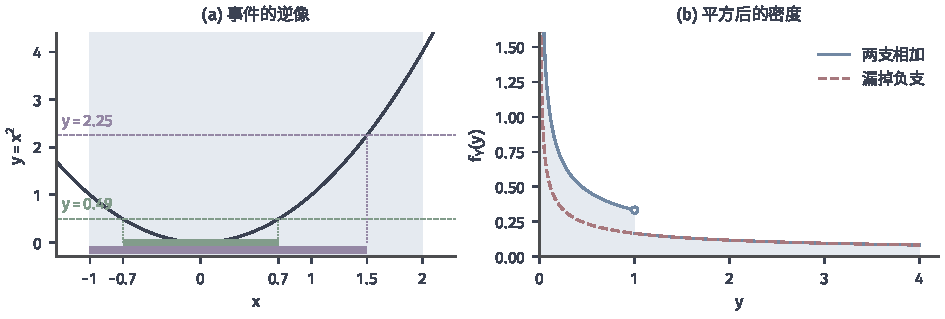
\includegraphics[width=160mm]{figures/01-basic-mathematics/05-probability-and-statistics-basics/matplotlib/prob-square-transform/figure.pdf}
  \caption{$X\sim\operatorname{U}(-1,2)$经平方$Y=X^2$的变换。(a)浅色竖带是$X$的取值范围；水平虚线是两个阈值$y$，横轴附近的粗线是事件$\{Y\leq y\}$在$X$轴上的逆像：$y=0.49$时为对称区间$[-0.7,0.7]$，$y=2.25$时左端被取值范围截断为$[-1,1.5]$。(b)$Y$的密度：在$(0,1)$上两支逆像都有贡献，密度为$1/(3\sqrt y)$；在$(1,4)$上只剩正支，密度为$1/(6\sqrt y)$，因而在$y=1$处跳降。虚线是遗漏负支时得到的错误曲线，它在$(0,1)$上少了一半，总面积只有$2/3$。}
  \label{fig:prob-square-transform}
\end{figure*}

\subsection{平移、缩放与标准化}
\label{sec:prob-standardization}

\paragraph{仿射变换的分布}
改变单位、零点或符号，都是对随机变量作仿射变换$Y=aX+b$。它是最简单的变换，也是比较不同变量、使用分布表时最常用的一步。

设$a>0$，则$aX+b\leq y$等价于$X\leq(y-b)/a$，所以$F_Y(y)=F_X\bigl((y-b)/a\bigr)$。设$a<0$，不等号方向反转，$F_Y(y)=\mathbb{P}\bigl(X\geq(y-b)/a\bigr)=1-F_X\bigl(((y-b)/a)^-\bigr)$。若$X$有密度，由定理~\ref{thm:prob-density-change}（$h(y)=(y-b)/a$，$|h'(y)|=1/|a|$）
\[
  f_Y(y)=\frac{1}{|a|}f_X\Bigl(\frac{y-b}{a}\Bigr).
\]
密度的形状不变，只是沿横轴平移、伸缩或翻转，高度同时按$1/|a|$调整以保持总面积为$1$。均值与方差按第~\ref{sec:prob-variance}节的公式变化：$\mathbb{E}[Y]=a\,\mathbb{E}[X]+b$，$\operatorname{Var}(Y)=a^2\operatorname{Var}(X)$。

例如$Z\sim\mathcal{N}(0,1)$时，$Y=\sigma Z+\mu$（$\sigma>0$）的密度是$\frac1\sigma\varphi\bigl(\frac{y-\mu}{\sigma}\bigr)$，正是$\mathcal{N}(\mu,\sigma^2)$；这验证了第~\ref{sec:prob-gaussian}节的说法。更一般地，$X\sim\mathcal{N}(\mu,\sigma^2)$且$a\neq0$时，$aX+b\sim\mathcal{N}(a\mu+b,a^2\sigma^2)$：高斯分布族在仿射变换下封闭。

$a=0$是退化情形：$Y=b$恒为常数，分布函数在$b$处从$0$跳到$1$，即使$X$有密度，$Y$也没有密度，方差为$0$。上面带$1/|a|$的密度公式在这里失效，因为所有概率都被压到了一个点上。

\paragraph{标准化}
比较不同单位、不同尺度的量时，我们常把它们换算到共同的尺度。设$X$的方差有限且$\sigma^2=\operatorname{Var}(X)>0$，均值为$\mu$。

\begin{definition}[标准化]
\label{def:prob-standardization}
称
\[
  Z=\frac{X-\mu}{\sigma}
\]
为$X$的\term{标准化}（standardization）变量。
\end{definition}

由仿射变换的公式，$\mathbb{E}[Z]=0$，$\operatorname{Var}(Z)=1$。$Z$的取值表示“偏离均值多少个标准差”，与原来的单位无关。例如两门考试的平均分与离散程度不同，一名学生在甲考试得$85$分（均值$70$、标准差$10$），在乙考试得$80$分（均值$60$、标准差$8$），标准化值分别为$1.5$与$2.5$，乙考试的相对表现更好。第~\ref{sec:prob-gaussian}节的概率计算，也正是先把高斯变量标准化，再查$\Phi$的表。

标准化只改变位置与尺度，不改变分布的形状。高斯变量标准化后是$\mathcal{N}(0,1)$，这是高斯族在仿射变换下封闭的结果；其他分布标准化后并不会变成高斯分布。$T\sim\operatorname{Exp}(1)$标准化后$Z=T-1$，取值于$[-1,\infty)$，偏度仍为$2$；$\operatorname{Bernoulli}(p)$标准化后仍只取两个值。事实上，$a>0$时偏度与峰度在仿射变换下不变，因为分子与分母中的$a$的幂次相互抵消。因此，“零均值、单位方差”与“服从标准正态分布”是两回事，使用$\Phi$的表之前必须另有理由相信变量服从或近似服从高斯分布。

\section{本章小结}
\label{sec:prob-summary}

回到章首的三个问题。掷骰子时，样本空间是$\{1,\dots,6\}$，“出现偶数点”是子集$\{2,4,6\}$，在等可能假设下其概率为$1/2$。抽检问题在“每个$10$件子集等可能”的假设下由计数求得：不放回时至少一件次品的概率约为$0.416$；若改为有放回，次品数服从二项分布，概率约为$0.401$，次品数的均值都是$0.5$。等待时间问题若采用平均$5$分钟的指数模型，等待超过$10$分钟的概率约为$0.135$，中位数约$3.5$分钟。每个答案都依赖明确的模型假设：等可能性、独立性或无记忆性，一旦假设改变，计算就要随之调整。

本章的对象之间有清楚的层次。概率给事件赋值，并由三条规则推出补事件、加法公式与连续性；条件概率与独立性描述已知信息怎样改变概率。随机变量把结果对应为数值，它的分布汇总了“取值落在哪里”的全部概率，可以统一用分布函数表示；离散变量还可以用质量函数逐点列出，有密度的变量则用密度积分计算，两者之外还有混合分布等情形。

完整分布与数值特征回答不同的问题。分布能计算任何取值范围的概率，例如等待超过$10$分钟的概率；期望、方差与分位数则把分布压缩成几个数，分别回答平均位置、波动大小与“多少比例不超过某个值”。数值特征便于报告和比较，但不能代替分布：相同的均值与方差可以对应形状截然不同的分布，均值也可能根本不存在。常见分布族由少数参数和明确的假设确定，二项与Poisson、几何与指数之间的关系说明了这些模型怎样相互联系。变换一节则说明，新变量的分布可以由原分布推前得到，计算时要先确定取值范围，并收齐所有逆像分支。

本章始终只看一个随机变量。实际问题中，我们往往同时关心几个量：抽检样本中两类缺陷各有几件、同一顾客的等待时间与服务时间、多次测量的读数。它们如何共同变化，知道一个之后另一个的分布怎样改变，它们的和与比值服从什么分布，是第~\ref{chap:random-vectors}章要回答的问题。
